\documentclass[12pt]{article}
\usepackage{fullpage}
\usepackage{microtype}
\usepackage{multirow}
\usepackage{amsmath, amsfonts, amssymb, amsthm}
\usepackage{mathtools}
\usepackage{bm}
\usepackage{tikz}
\usepackage{algorithm}
\usepackage{algpseudocode}
\usepackage{verbatim}
\usepackage{hyperref}
\usepackage{subcaption}
\usepackage{cleveref}
\usepackage[sort]{natbib}
\usepackage{complexity}
\usepackage{authblk}
\usepackage{enumerate}
\usepackage{adjustbox}
\usepackage{xurl}
\usepackage{array}

\usetikzlibrary{arrows}
\usetikzlibrary{shapes}

\newcommand{\prob}[1]{\mathbb{P}(#1)}
\newcommand{\varprob}[1]{\mathbb{P}\left(#1\right)}

\newcommand{\argmax}{\operatorname{argmax}}
\newcommand{\argmin}{\operatorname{argmin}}
\newcommand{\true}{\operatorname{true}}
\newcommand{\false}{\operatorname{false}}
\newcommand{\sharpp}{\#\P}
\newcommand{\return}[1]{\textbf{return }#1}
\newcommand{\RR}{\mathcal{R}}
\newcommand{\CPP}{C\nolinebreak[4]\hspace{-.05em}\raisebox{.22ex}{\footnotesize\bf ++}}
\newcommand{\package}[2]{\texttt{#1}~\citep{#2}}
\newcommand{\idx}{\iota}
\newcommand{\ind}[1]{\mathbf{1}(#1)}
\newcommand{\dual}[1]{#1_{\operatorname{op}}}

\newcommand{\incomp}[1][]{\|_{#1}}
\newcommand{\mat}[1]{\mathbf{M}(#1)}

\newcommand{\dset}[2][]{\operatorname{down}_{#1}(#2)}
\newcommand{\uset}[2][]{\operatorname{up}_{#1}(#2)}
\newcommand{\pset}[2][]{\operatorname{pred}_{#1}(#2)}
\newcommand{\sset}[2][]{\operatorname{succ}_{#1}(#2)}

\newcommand{\eord}{{\preceq_{\varnothing}}}
\newcommand{\iord}{{\preceq_{\hat{\mathcal{I}}}}}
\newcommand{\pord}{{\leqslant_{\theta}}}
\newcommand{\phord}{{\leqslant_{\hat{\theta}}}}
\newcommand{\rord}[1][\mathbf{r}]{{\leqslant_{#1}}}

\newcommand{\iords}{{\prec_{\hat{\mathcal{I}}}}}
\newcommand{\rords}[1][\mathbf{r}]{{<_{#1}}}

\newcommand{\iordn}{{\preceq_{\hat{\mathcal{I}}_{n}}}}

\newcommand{\preceqr}[1]{{\preceq\restriction_{#1}}}
\newcommand{\leqslantr}[1]{{\leqslant\restriction_{#1}}}

\newcommand{\rankp}{{\mathbf{r}_\theta}}
\newcommand{\ranks}{{\mathbf{r}_{\hat{\theta}}}}
\newcommand{\ranksn}{{\mathbf{r}_{\hat{\theta}_n}}}

\newcommand{\LE}[1]{\operatorname{LE}(#1)}
\newcommand{\WE}[1]{\operatorname{WE}(#1)}

\newcommand{\keywordname}{\textbf{Keywords:}}
\newcommand{\keywords}[1]{\par\addvspace\baselineskip\noindent\keywordname\enspace\ignorespaces#1}

\newcommand{\dataUncertainty}{\ensuremath{0.534}}
\newcommand{\dataSubsetUncertainty}{\ensuremath{0.498}}
\newcommand{\dataRankDistance}{\ensuremath{0.091}}


\newtheorem{theorem}{Theorem}
\numberwithin{theorem}{section}
\newtheorem{definition}[theorem]{Definition}
\newtheorem{lemma}[theorem]{Lemma}
\newtheorem{corollary}[theorem]{Corollary}
\newtheorem{conjecture}[theorem]{Conjecture}
\newtheorem{question}[theorem]{Question}

\defcitealias{oeisA000670}{OEIS A000670\nocite{oeisA000670}}

\begin{document}

\title{An Order-Theoretic Perspective on Rank Estimation}
\author{Justin Rising\thanks{email: \texttt{jkrising@gmail.com}}\\Boston, MA}
\maketitle

\begin{abstract}
The ranks of estimated parameters are themselves estimates of the population ranks and are therefore uncertain.  As they are deterministic functions of the estimated parameters, their uncertainty is completely determined by the uncertainty in those parameter estimates.  Here I give a characterization of this relationship using notions from the subfield of combinatorics known as order theory.  I use this relationship to develop a general theory of rank estimation that remains valid even when the parameters to be ranked are not necessarily distinct.  I then develop methods for set estimation, point estimation and uncertainty quantification based on the theory, and I apply these methods to real and simulated data to study their behavior.  I provide these methods through an \texttt{R} package to facilitate further experiments.
\end{abstract}

\section{Introduction}
\label{sec_intro}

Estimating the ranks of unknown parameters is a fundamental statistical problem with applications in every field that works with data.  When faced with this problem, practitioners typically report the sample ranks of the point estimates with no associated measure of uncertainty.  However, as shown in~\cite{hall2010variability} and~\cite{zuk2007uncertainty}, sample ranks are highly sensitive to measurement noise, so simply reporting a point estimate can vastly overstate how certain we are regarding its value.

This problem has been recognized at least since~\cite{goldstein1996tables} and has attracted a reasonable amount of attention (see~\cite{almohamad2022rankCIs} for a recent survey).  The majority of the literature has concentrated on interval estimates for the individual ranks, but recently a joint confidence set for the population ranking was proposed in~\cite{klein2020jointCR}.  The main idea there is that a collection of interval estimates that cover the true parameters contain some information about their order.  If we are given the set of interval estimates shown in Figure~\ref{fig_example}, then conditional on the event that $\theta_j \in \hat{I}_j$ for all $j$, we know that $\theta_1 < \theta_3$, but we cannot draw any inferences about the rank of $\theta_2$.

\begin{figure}[t]
\centering
% !TEX encoding = UTF-8 Unicode
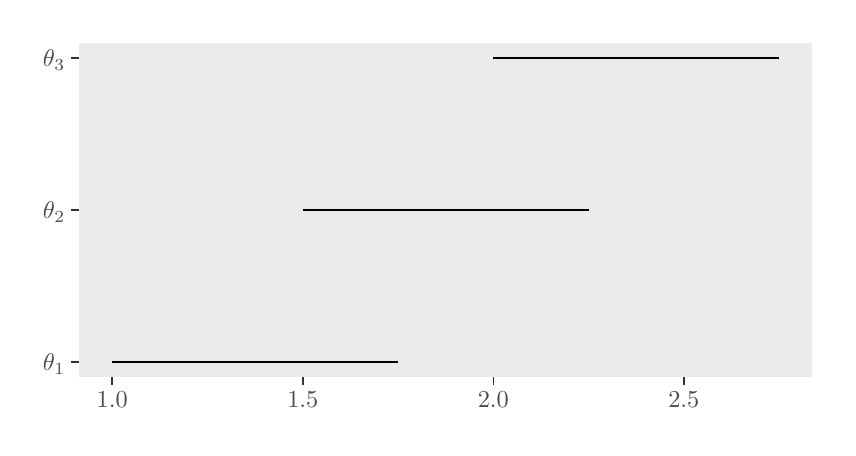
\begin{tikzpicture}[x=1pt,y=1pt]
\definecolor{fillColor}{RGB}{255,255,255}
\path[use as bounding box,fill=fillColor,fill opacity=0.00] (0,0) rectangle (289.08,144.54);
\begin{scope}
\path[clip] (  0.00,  0.00) rectangle (289.08,144.54);
\definecolor{drawColor}{RGB}{255,255,255}
\definecolor{fillColor}{RGB}{255,255,255}

\path[draw=drawColor,line width= 0.6pt,line join=round,line cap=round,fill=fillColor] (  0.00,  0.00) rectangle (289.08,144.54);
\end{scope}
\begin{scope}
\path[clip] ( 18.53, 18.22) rectangle (283.58,139.04);
\definecolor{fillColor}{gray}{0.92}

\path[fill=fillColor] ( 18.53, 18.22) rectangle (283.58,139.04);
\definecolor{drawColor}{RGB}{0,0,0}

\path[draw=drawColor,line width= 0.6pt,line join=round] ( 30.58, 23.71) -- (133.84, 23.71);

\path[draw=drawColor,line width= 0.6pt,line join=round] ( 99.42, 78.63) -- (202.69, 78.63);

\path[draw=drawColor,line width= 0.6pt,line join=round] (168.27,133.55) -- (271.53,133.55);
\end{scope}
\begin{scope}
\path[clip] (  0.00,  0.00) rectangle (289.08,144.54);
\definecolor{drawColor}{gray}{0.30}

\node[text=drawColor,anchor=base east,inner sep=0pt, outer sep=0pt, scale=  0.88] at ( 13.58, 20.68) {$\theta_1$};

\node[text=drawColor,anchor=base east,inner sep=0pt, outer sep=0pt, scale=  0.88] at ( 13.58, 75.60) {$\theta_2$};

\node[text=drawColor,anchor=base east,inner sep=0pt, outer sep=0pt, scale=  0.88] at ( 13.58,130.52) {$\theta_3$};
\end{scope}
\begin{scope}
\path[clip] (  0.00,  0.00) rectangle (289.08,144.54);
\definecolor{drawColor}{gray}{0.20}

\path[draw=drawColor,line width= 0.6pt,line join=round] ( 15.78, 23.71) --
	( 18.53, 23.71);

\path[draw=drawColor,line width= 0.6pt,line join=round] ( 15.78, 78.63) --
	( 18.53, 78.63);

\path[draw=drawColor,line width= 0.6pt,line join=round] ( 15.78,133.55) --
	( 18.53,133.55);
\end{scope}
\begin{scope}
\path[clip] (  0.00,  0.00) rectangle (289.08,144.54);
\definecolor{drawColor}{gray}{0.20}

\path[draw=drawColor,line width= 0.6pt,line join=round] ( 30.58, 15.47) --
	( 30.58, 18.22);

\path[draw=drawColor,line width= 0.6pt,line join=round] ( 99.42, 15.47) --
	( 99.42, 18.22);

\path[draw=drawColor,line width= 0.6pt,line join=round] (168.27, 15.47) --
	(168.27, 18.22);

\path[draw=drawColor,line width= 0.6pt,line join=round] (237.11, 15.47) --
	(237.11, 18.22);
\end{scope}
\begin{scope}
\path[clip] (  0.00,  0.00) rectangle (289.08,144.54);
\definecolor{drawColor}{gray}{0.30}

\node[text=drawColor,anchor=base,inner sep=0pt, outer sep=0pt, scale=  0.88] at ( 30.58,  7.21) {1.0};

\node[text=drawColor,anchor=base,inner sep=0pt, outer sep=0pt, scale=  0.88] at ( 99.42,  7.21) {1.5};

\node[text=drawColor,anchor=base,inner sep=0pt, outer sep=0pt, scale=  0.88] at (168.27,  7.21) {2.0};

\node[text=drawColor,anchor=base,inner sep=0pt, outer sep=0pt, scale=  0.88] at (237.11,  7.21) {2.5};
\end{scope}
\end{tikzpicture}

\caption{A simple example illustrating the main idea.}
\label{fig_example}
\end{figure}

Since there are only finitely many rankings that can be obtained by picking one point from each interval, the problem is combinatorial.  In particular, we are dealing with order theory, a branch of combinatorics that studies relations that can be interpreted as orders as long as we do not require every pair of elements to be comparable.  Our first task will therefore be to describe the idea of~\cite{klein2020jointCR} in order-theoretic terms.  The key result is a characterization of the uncertainty in the estimated rank in terms of the uncertainty in the estimated parameters.  This order-theoretic perspective enables us to develop a theory of rank estimation, and I will show how it can be applied to form point estimates and set estimates of the population ranking and to quantify the uncertainty in these estimates.

Many of the methods that have been developed for problems related to rank estimation so far fail in the case where the unknown parameters are not necessarily distinct~\citep{hall2009bootstrap, xie2009ties}.  The solutions that have been proposed come with the correct theoretical guarantees but do not follow from any more general theory.  The order-theoretic perspective, on the other hand, allows us to see this case as a minor variation of the case where the parameters are equal, and the methods that we develop will work in either case.

While I believe that this represents a significant advance, the material in this paper is by no means the last word on any of the problems involved in rank estimation.  We will not consider problems related to hypothesis testing or visualization (but see~\cite{fattore2014visualizing} for the latter).  In addition, the methods described here are the most obvious, and while they have nice theoretical properties, none of them clearly dominates other approaches.  In order to facilitate experimentation with these methods, implementations are provided in the \texttt{R} package \texttt{orderRanks}.

The remainder of this paper is laid out as follows.  First in section~\ref{sec_bkgd} we will discuss the necessary order-theoretic concepts and vocabulary for the remainder of the paper.  Then in sections~\ref{sec_theory} and~\ref{sec_rank_int} we will develop the basic theory that will inform all subsequent discussions.  In sections~\ref{sec_conf_set},~\ref{sec_point_est} and~\ref{sec_uncert_quant} we will see how the theory applies to the problems of set estimation, point estimation and uncertainty quantification respectively and then derive methods for all of these problems.  Finally in sections~\ref{sec_sim} and~\ref{sec_data} we will discuss the results of applying those methods to both simulated and real data with an emphasis on possible directions for future research.

\section{An Incomplete Introduction to Order Theory}
\label{sec_bkgd}

We begin with a survey of the order-theoretic concepts that will be used in the remainder of this paper.  Here we will discuss the concepts that are used throughout the paper; notions which are only used in one section will be defined as needed.  This survey is intentionally limited to the topics that are relevant to this paper; for a more comprehensive introduction, see~\cite{schroder2016posetBook}.

Let $[n]$ denote a set with $n$ elements.  A partial order $\preceq$ is a relation on $[n]$ such that the following hold for all $j_1, j_2, j_3 \in [n]$:

\begin{enumerate}

\item $j_1 \preceq j_1$.

\item $j_1 \preceq j_2$ and $j_2 \preceq j_1$ implies $j_1 = j_2$.

\item $j_1 \preceq j_2$ and $j_2 \preceq j_3$ implies $j_1 \preceq j_3$.

\end{enumerate}

\noindent
These properties are respectively referred to as reflexivity, antisymmetry and transitivity.  The pair $([n], \preceq)$ is referred to as an ordered set.

When $j_1 \preceq j_2$ and $j_1 \neq j_2$, we write $j_1 \prec j_2$.  When neither $j_1 \preceq j_2$ nor $j_2 \preceq j_1$, we say that $j_1$ and $j_2$ are incomparable and write $j_1 \incomp j_2$.  An order in which every pair of elements is comparable is referred to as a linear order.  The order in which no two distinct elements are comparable is known as the empty order and is denoted as $\eord$.  
The dual of an order $\preceq$, denoted $\dual{\preceq}$, is the order such that $j_1 \dual{\preceq} j_2$ if and only if $j_2 \preceq j_1$.

If the relation $\incomp$ is transitive we say that $\preceq$ is a weak order.  These orders capture the idea of a linear order with ties.  Every linear order is a weak order, but so is the empty order.  We will use $\leqslant$ to denote a weak order and note in text when that denotes a linear order.

If $\preceq_1$ and $\preceq_2$ are orders on $[n]$ such that $j_1 \preceq_1 j_2$ implies $j_1 \preceq_2 j_2$, $\preceq_2$ is said to be an extension of $\preceq_1$.  An extension of an order which is linear is a linear extension, and an extension which is weak is a weak extension.  The set of linear extensions of $\preceq$ is denoted by $\LE{\preceq}$ and the set of weak extensions by $\WE{\preceq}$.

Given $j_1 \in [n]$, we define $\dset{j_1} = \{j_2 \in [n] \mid j_2 \preceq j_1\}$ and $\uset{j_1} = \{j_2 \in [n] \mid j_1 \preceq j_2\}$.  We then define $\pset{j_1} = \dset{j_1} \setminus \{j_1\}$ and $\sset{j_1} = \uset{j_1} \setminus \{j_1\}$.  These sets are respectively referred to as the down set, up set, predecessor set and successor set of $j_1$.  We define the interval $[j_1, j_2]$ to be $\uset{j_1} \cap \dset{j_2}$.

When we are considering multiple orders, we will augment the notation here with subscripts to distinguish between them.  Thus $\dset[\preceq_1]{j_1}$ is the down set of $j_1$ with respect to $\preceq_1$, $\incomp[\preceq_2]$ is the incomparability relationship of $\preceq_2$, and so on and so forth.

Formally, an order $\preceq$ is a subset of $[n] \times [n]$ and $j_1 \preceq j_2$ is shorthand for $(j_1, j_2) \in \preceq$.  This definition is essential for understanding the following theorem:

\begin{theorem}[\cite{dushnik1941posets}]
\label{thm_lin_ext_int}
$\preceq$ is the intersection of its linear extensions.
\end{theorem}

\noindent
We can also identify an order $\preceq$ with the matrix $\mat{\preceq}$ defined by $[\mat{\preceq}]_{ij} = \ind{i \preceq j}$.

We are interested in order properties that are determined by a set of interval estimates, so we will primarily concern ourselves with the class of orders known as interval orders.  Given an interval $I$, we will write $\ell(I)$ and $r(I)$ to denote its left and right endpoints respectively.  Given a set of open intervals $\mathcal{I} = \{I_1, \dots, I_n\}$, we will define an order $\preceq_\mathcal{I}$ on $[n]$ by $j_1 \preceq_\mathcal{I} j_2$ if and only if $r(I_{j_1}) \leq \ell(I_{j_2})$.  An order that can be realized in this fashion is said to be an interval order.  We will refer to $\preceq_\mathcal{I}$ as the order generated by $\mathcal{I}$ and we will refer to $\mathcal{I}$ as a representation of $\preceq_\mathcal{I}$.  Every weak order is an interval order, but the converse is false; see Figure~\ref{fig_example} for a counterexample.

Interval orders have an order-theoretic characterization which we record this as Theorem~\ref{thm_int_ord_char}, and the subsequent analysis is informed heavily by a related fact which we capture in Corollary~\ref{cor_int_ord_card}.  The proof of Corollary~\ref{cor_int_ord_card} is straightforward and is omitted.

\begin{theorem}[\cite{trotter1997intervalOrder}]
\label{thm_int_ord_char}
An order $\preceq$ is an interval order if and only if $\{\pset[\preceq]{j}\}$ is linearly ordered by set inclusion.
\end{theorem}

\begin{corollary}
\label{cor_int_ord_card}
If $\preceq$ is an interval order then $|\pset{j_1}| = |\pset{j_2}|$ if and only if $\pset{j_1} = \pset{j_2}$.
\end{corollary}
\begin{proof}
Clearly if $\pset{j_1} = \pset{j_2}$ then $|\pset{j_1}| = |\pset{j_2}|$.  If $|\pset{j_1}| = |\pset{j_2}|$ but $\pset{j_1} \neq \pset{j_2}$ then $\pset{j_1} \nsubseteq \pset{j_2}$ and $\pset{j_2} \nsubseteq \pset{j_1}$, violating Theorem~\ref{thm_int_ord_char}.
\end{proof}

\noindent
The dual of the order generated by a set of intervals is the order generated by the image of those intervals under the map $x \mapsto -x$ and is therefore also an interval order.  As a result, there are analogues to Theorem~\ref{thm_int_ord_char} and Corollary~\ref{cor_int_ord_card} for successor sets as well.


\section{The Main Theorem}
\label{sec_theory}

Now that we have finished with the necessary background material, we can move on to the main discussion.  We begin with a statement of the problem we are considering, introduce the necessary vocabulary, and state and prove the main theorem which will be used for all of the subsequent discussion.

Given a set of points $x_1, \dots, x_n$, the rank of $x_j$ is denoted by $r_j(x_1, \dots, x_n)$ and is equal to $1 + \sum_{i = 1}^n \ind{x_i < x_j}$.  The vector whose $j$th entry is $r_j(x_1, \dots, x_n)$ is referred to as a ranking and is denoted by $\mathbf{r}(x_1, \dots, x_n)$.  If all of the points $x_1, \dots, x_n$ are distinct, we will say that $\mathbf{r}(x_1, \dots, x_n)$ has no ties.  When the data is clear from context, we will write its ranking as $\mathbf{r}$.

We consider the problem of drawing inferences about the ranks of an unknown set of parameters $\theta_1, \dots, \theta_p$.  We assume that we have consistent point estimates $\hat{\theta}_1, \dots, \hat{\theta}_p$ and open interval estimates $\hat{I}_1, \dots, \hat{I}_p$.  We will denote the set of interval estimates as $\hat{\mathcal{I}}$.

The population ranking $\rankp$ is defined to be $\mathbf{r}(\theta_1, \dots, \theta_p)$ and the sample ranking $\ranks$ is defined to be $\mathbf{r}(\hat{\theta}_1, \dots, \hat{\theta}_p)$.  The sample ranking is a consistent estimator of the population ranking because the point estimates are consistent, but as the point estimates are inexact, the sample ranking is as well.  Because the sample ranking is determined by the point estimates and the uncertainty in those estimates is described by the interval estimates, the uncertainty in the sample ranking is somehow determined by the interval estimates.  Our goal here is to describe that relationship, and we will now develop the machinery to do so.

We say that a ranking $\mathbf{r}$ is compatible with the interval estimates if there is a set of points $x_1, \dots, x_p$ such that $x_j \in \hat{I}_j$ for all $j$ and $\mathbf{r} = \mathbf{r}(x_1, \dots, x_p)$.  The interval estimates consist of plausible values of the parameters given the data we have and the decision procedures we have chosen, so the rankings that are compatible with them are the plausible rankings based on the same criteria.

If $\hat{\theta}_j \in \hat{I}_j$ for all $j$ then the sample ranking is compatible with the interval estimates, but if any two interval estimates overlap others will be as well.  We therefore face the problem of describing the set of rankings that are compatible with the interval estimates.  In order to do so, we must first introduce two classes of orders on $[p]$ and one further piece of vocabulary.

First, given a ranking $\mathbf{r} \in \mathbb{R}^p$, we define $\rord$ to be the weak order such that $j_1 \rord j_2$ whenever $j_1 = j_2$ or $r_{j_1} < r_{j_2}$.  We will refer to $\rord$ as the order generated by $\mathbf{r}$.  We will define the parameter order $\pord$ to be $\rord[\rankp]$.  Second, given the set of interval estimates $\hat{\mathcal{I}}$, we will define the order $\iord$ to be the interval order generated by these estimates.  We will refer to $\iord$ as the \emph{sample interval order}.

Finally, let $\mathbf{r}$ be a ranking and $\mathcal{I}$ a set of intervals.  If $\rord$ is not a weak extension of $\preceq_{\mathcal{I}}$, then there is some pair $(j_1, j_2)$ such that $r_{j_2} \leq r_{j_1}$ and $r(I_{j_1}) \leq \ell(I_{j_2})$.  We will refer to such a pair as an \emph{inversion} with respect to $\preceq_{\mathcal{I}}$.

We can now give the characterization of rankings that are compatible with the interval estimates.  We record this result as Theorem~\ref{thm_main}

\begin{theorem}
\label{thm_main}
A ranking $\mathbf{r}$ is compatible with the interval estimates if and only if $\rord$ is a weak extension of $\iord$.
\end{theorem}
\begin{proof}
Suppose that $\mathbf{r}$ is compatible with the interval estimates.  If there are no $j_1, j_2$ such that $j_1 \iords j_2$, then $\rord$ is a weak extension of $\iord$ because every order is an extension of $\iord$.  If $j_1 \prec j_2$, then $r(\hat{I}_{j_1}) < \ell(\hat{I}_{j_2})$.  Since $x_{j_1} \in \hat{I}_{j_1}$ and $x_{j_2} \in \hat{I}_{j_2}$, we must have $x_{j_1} \leq r(\hat{I}_{j_1})$ and $\ell(\hat{I}_{j_2}) \leq x_{j_2}$.  Therefore $x_{j_1} < x_{j_2}$ and $j_1 \rords j_2$, so $\rord$ is a weak extension of $\iord$.

Now suppose that $\rord$ is a weak extension of $\iord$.  Let $v_1, \dots, v_m$ be the distinct values of $\mathbf{r}$ in increasing order, let $\tilde{I}_j = \cap\{\hat{I}_k \mid r_k = v_j\}$, and let $\epsilon$ be the smallest distance between two distinct endpoints of the interval estimates.  Let $u_1 = \ell(\tilde{I}_1) + \epsilon / 2p$ and define $u_{k + 1} = \max(u_k, \ell(\tilde{I}_{k + 1})) + \epsilon / 2p$.  Because $\rord$ is a weak extension of $\iord$, there is no inversion with respect to the order generated by $\{\tilde{I}_j\}$ and this implies that $u_j \leq r(\tilde{I}_k)$ whenever $j \leq k$.  Furthermore, the difference between $u_j$ and the nearest right endpoint is at least $\epsilon / 2$, so we have $u_j \in \tilde{I}_j$ for all $j$.

Finally we define $x_1, \dots, x_p$ by $x_j = u_{r_j}$.  We have that $\mathbf{r}(x_1, \dots, x_p) = \mathbf{r}$ by construction and $x_j \in \hat{I}_j$ because $u_j \in \tilde{I}_j$.  Therefore $\mathbf{r}$ is compatible with the interval estimates.
\end{proof}

A ranking $\mathbf{r}$ is generated by distinct points and therefore has no ties if and only if $\rord$ is a linear order.  Therefore we have the following corollary of Theorem~\ref{thm_main}.

\begin{corollary}
\label{cor_main}
If $\mathbf{r}$ has no ties, $\mathbf{r}$ is compatible with the interval estimates if and only if $\rord$ is a linear extension of $\iord$.
\end{corollary}

Theorem~\ref{thm_main} does not hold if we allow pairs of intervals to intersect in a single point.  Our assumption that the interval estimates are open rules this out.

\section{Rank Intervals}
\label{sec_rank_int}

Here we continue our development of the theory by introducing the notion of rank intervals.  These intervals were used as confidence intervals for the population ranks in~\cite{klein2020jointCR}, but as we will see they are useful more generally.  We will begin by defining the rank intervals in order-theoretic terms, discuss how to compute them efficiently, and finally show that they are a natural generalization of the idea of a rank to interval orders.

\subsection{Basic Definitions and Results}
\label{subsec_rank_int_basics}

We begin by generalizing the definition of ranks we gave in section~\ref{sec_theory} to arbitrary weak orders.  If $\leqslant$ is a weak order on $[p]$, we define the rank of $j$ with respect to $\leqslant$, denoted as $r_\leqslant(j)$, to be $\sum_{i = 1}^n \ind{i \leqslant j}$.  Given a partial order $\preceq$ on $[p]$, we can then define the rank set of $j$ as the set of values $r_\leqslant(j)$ such that $\leqslant$ is a weak extension of $\preceq$.  We note, however, that if $\preceq$ has a weak extension $\leqslant$ such that $r_\leqslant(j) = r$, then it has a linear extension that assigns rank $r$ to $j$ as well.  Therefore when defining the rank sets of $\preceq$ it is sufficient to consider the linear extensions of $\preceq$.

We will show in Theorem~\ref{thm_rank_int} that the rank set of $j$ with respect to $\preceq$ is an interval (but in $\mathbb{Z}$ rather than $\mathbb{R}$).  In light of this result, we will refer to it as the rank interval of $j$ with respect to $\preceq$ and denote it as $I_\preceq(j)$.

\begin{theorem}
\label{thm_rank_int}
$I_\preceq(j) = [|\dset{j}|, p + 1 - |\uset{j}|]$.
\end{theorem}
\begin{proof}
If $j_1 \preceq j$ and $\leqslant$ is a linear extension of $\preceq$, then we must have $r_\leqslant(j_1) \leq r_\leqslant(j)$.  Therefore $r_\leqslant(j) \geq |\dset{j}|$.  Applying the same argument to $\dual{\preceq}$ allows us to conclude that $r_\leqslant(j) \leq n + 1 - |\uset{j}|$.  $j$ is incomparable to any value outside of $\dset{j} \cup \uset{j}$, so its rank can be in any position between the bounds we have previously established.
\end{proof}

We will have need of an alternative description of a rank interval which we record as Corollary~\ref{cor_rank_int_alt}.  The proof is straightforward and is omitted.

\begin{corollary}
\label{cor_rank_int_alt}
$I_\preceq(j) = [|\pset{j}| + 1, p - |\sset{j}|]$.
\end{corollary}

Given an interval order $\preceq$, we define $P_j = \{\pset{j^{'}} \mid \pset{j^{'}} \subset \pset{j}\}$ and $S_j = \{\sset{j^{'}} \mid \sset{j} \subset \sset{j^{'}}\}$.  Following~\cite{mitas1994semiRep}, we observe that the intervals $I_j = (|P_j| - \epsilon, |S_j| + \epsilon)$ are a representation of $\preceq$ when $\epsilon \in (0, 1/2)$.  From this result and Corollaries~\ref{cor_int_ord_card} and~\ref{cor_rank_int_alt} we can prove that the rank intervals of an interval order uniquely describe it, and we record this result as Theorem~\ref{thm_rank_int_equal}.

\begin{theorem}
\label{thm_rank_int_equal}
Two interval orders $\preceq_1$ and $\preceq_2$ are equal if and only if $I_{\preceq_1}(j) = I_{\preceq_2}(j)$ for all $j$.
\end{theorem}

We now consider how the rank intervals of related orders are structured.  We say that $\preceq_2$ is rank compatible with $\preceq_1$ if $I_{\preceq_2}(j) \subseteq I_{\preceq_1}(j)$ for all $j$.  We will show that the extensions of an order are always rank compatible with it.

\begin{theorem}
\label{thm_rank_compat}
If $\preceq_2$ is an extension of $\preceq_1$, then $\preceq_2$ is rank compatible with $\preceq_1$.
\end{theorem}
\begin{proof}
Because $\preceq_2$ is an extension of $\preceq_1$, we have $\pset[\preceq_1]{j} \subseteq \pset[\preceq_2]{j}$ and $\sset[\preceq_1]{j} \subseteq \sset[\preceq_2]{j}$.  The result follows from Corollary~\ref{cor_rank_int_alt}.
\end{proof}

Theorem~\ref{thm_rank_compat} implies that the ranks of any weak extension of $\preceq$ are contained in its rank intervals.  We will give this result in Corollary~\ref{cor_weak_ord_rank_compat}, but we first give an alternative description of the ranks of a weak order that will be useful later.

\begin{lemma}
\label{lem_weak_rank_dset}
If $\leqslant$ is a weak order, then $r_\leqslant(j) = |\dset{j}|$.
\end{lemma}

\begin{corollary}
\label{cor_weak_ord_rank_compat}
If $\leqslant$ is a weak extension of $\preceq$, then $r_\leqslant(j) \in I_\preceq(j)$ for all $j$.
\end{corollary}
\begin{proof}
This follows from Lemma~\ref{lem_weak_rank_dset} and Theorem~\ref{thm_rank_compat}.
\end{proof}

\begin{table}[t]
\centering
\begin{tabular}{|c|c|c|}
\hline
$j$&$r_\leqslant(j)$&$I_\preceq(j)$\\
\hline
$j_1$&$3$&$[1, 3]$\\
$j_2$&$4$&$[1, 4]$\\
$j_3$&$1$&$[1, 5]$\\
$j_4$&$2$&$[2, 5]$\\
$j_5$&$5$&$[3, 5]$\\
\hline
\end{tabular}
\caption{The counterexample to the converse of Corollary~\ref{cor_weak_ord_rank_compat}.}
\label{tab_rank_int_counter}
\end{table}

We might hope that the converse of Corollary~\ref{cor_weak_ord_rank_compat} is true.  Unfortunately this is not the case.  Consider the order on the set $\{j_1, \dots, j_5\}$ given by $j_1 \prec j_4$, $j_1 \prec j_5$ and $j_2 \prec j_5$.  The linear order defined by $j_3 \leqslant j_4 \leqslant j_1 \leqslant j_2 \leqslant j_5$ is rank compatible with $\preceq$ but is not a linear extension because it has $j_4 \leqslant j_1$ while $j_1 \prec j_4$.  See Table~\ref{tab_rank_int_counter} for the rank intervals of $\preceq$.

\subsection{Computing the Rank Intervals of the Sample Interval Order}
\label{subsec_rank_int_compute}

The rank intervals of $\iord$ will be used in all of the methods we will consider so we will now describe how to compute them efficiently.  While they can be computed from the row and column sums of $\mat{\iord}$, this requires us to compare every pair of elements directly.  By exploiting transitivity, we can instead compute the rank intervals with a single pass over the sorted endpoints of the interval estimates.  The method to do so is given in Algorithm~\ref{algo_rank_int}, and we analyze its correctness and performance in Theorem~\ref{thm_algo_rank_int}.

\begin{theorem}
\label{thm_algo_rank_int}
Algorithm~\ref{algo_rank_int} computes the rank intervals of $\iord$ with time complexity $O(p\log(p))$ and space complexity $O(p)$.
\end{theorem}
\begin{proof}
We begin by observing that $\pset{j} = \{j^{'} \mid r(I_{j^{'}} < \ell(I_j)\}$ and $\sset{j} = \{j^{'} \mid r(I_j) < \ell(I_{j^{'}}\}$.  Therefore by Corollary~\ref{cor_rank_int_alt}, if we can track the cardinalities of these sets, we can compute the rank intervals.  When we begin processing each value $v$, $c_r$ is updated the number of right endpoints which are less than the current value.  Therefore, for each $j \in S_\ell$, we have $|\pset{j}| = c_r$.  At the end of each iteration, $c_\ell$ is equal to the number of left endpoints which are less than or equal to the current value.  This equal to the difference between $p$ and the number of left endpoints which are greater than the current value, so for each $j \in S_r$ we have $c_\ell = p - |\sset{j}|$.

The running time of the algorithm is dominated by the cost of sorting the endpoints, and the extra space needed is dominated by the cost of storing the output.  We therefore have that the time complexity is $O(p\log(p))$ and the space complexity is $O(p)$.
\end{proof}

\begin{algorithm}[t]
\begin{algorithmic}
\Procedure{RankIntervals}{$\hat{I}_1, \dots, \hat{I}_p$}
  \State Let $V$ be a sorted list containing the elements of $\{\ell(\hat{I}_1), r(\hat{I}_1), \dots, \ell(\hat{I}_p), r(\hat{I}_p)\}$
  \State $c_\ell \gets 0$
  \State $c_r \gets 1$
  \For{$v \in V$}
    \State $S_\ell \gets \{j \mid \ell(I_j) = v\}$
    \State $S_r \gets \{j \mid r(I_j) = v\}$
    \State $c_r \gets c_r + |S_r|$
    \For{$j \in S_\ell$}
      \State $\ell(I_\iord(j)) \gets c_r$
    \EndFor
    \For{$j \in S_r$}
      \State $r(I_\iord(j)) \gets c_\ell$
    \EndFor
    \State $c_\ell \gets |S_\ell|$
  \EndFor
  \State $\return{\{I_\iord(j)\}}$
\EndProcedure
\end{algorithmic}
\caption{Compute the rank intervals of $\iord$.}
\label{algo_rank_int}
\end{algorithm}

\subsection{Rank Intervals as Ranks}
\label{subsec_rank_int_rank}

We close our discussion of rank intervals by arguing that the rank intervals of an interval order are the natural generalization of ranks beyond the class of weak orders.  We begin with a question: what does it mean for two elements of an ordered set to have the same rank?  Although there is a standard notion discussed in~\cite{stanley2011book}, it is only defined for a fairly special class of orders, and it fails to capture what I believe is the essence of a notion of rank.  In my opinion, when we say that two elements of an ordered set have the same rank, we mean that they are in some sense in the same position.  Our goal in the remainder of this section will be to make this intuition precise.

To do so, we will need the notion of an order automorphism.  If $(S_1, \preceq_1)$ and $(S_2, \preceq_2)$ are ordered sets, we say that a bijection $\phi : S_1 \rightarrow S_2$ is an order isomorphism when $s \preceq_1 t$ if and only if $\phi(s) \preceq_2 \phi(t)$.  An order automorphism is an order isomorphism where $S_1 = S_2$ and $\preceq_1 = \preceq_2$.

Let $\phi_{j_1j_2}$ denote a map from an ordered set to itself where $\phi_{j_1j_2}(j_1) = j_2$, $\phi_{j_1j_2}(j_2) = j_1$ and $\phi_{j_1j_2}(j) = j$ for all other $j$.  It is reasonable to say that $j_1$ and $j_2$ are in the same position exactly when $\phi_{j_1j_2}$ is an order automorphism, so we will say that they have the same rank in this case.  We will now state and prove a lemma that characterizes all pairs $j_1, j_2$ that have the same rank.

\begin{lemma}
\label{lem_aut}
$\phi_{j_1j_2}$ is an order automorphism if and only if $\pset{j_1} = \pset{j_2}$ and $\sset{j_1} = \sset{j_2}$.
\end{lemma}
\begin{proof}
Suppose that $\phi_{j_1j_2}$ is an order automorphism.  In this case, $j_1 \incomp j_2$, so $j \preceq j_1$ if and only if $j \preceq j_2$.  Therefore $\pset{j_1} = \pset{j_2}$.  A similar argument shows that $\sset{j_1} = \sset{j_2}$.

Now suppose that $\pset{j_1} = \pset{j_2}$ and $\sset{j_1} = \sset{j_2}$.  Then $j \preceq j_1$ if and only if j $\preceq j_2$, and $j_1 \preceq j$ if and only if $j_2 \preceq j$, so it follows that $\phi_{j_1j_2}$ is an order automorphism.
\end{proof}

We will now show that when $\preceq$ is an interval order, we can describe the pairs of elements that have the same rank in terms of the rank intervals.

\begin{theorem}
\label{thm_rank_int_rank}
If $\preceq$ is an interval order, then $\phi_{j_1j_2}$ is an order automorphism if and only if $I_\preceq(j_1) = I_\preceq(j_2)$.
\end{theorem}
\begin{proof}
This follows from Corollary~\ref{cor_int_ord_card}, Corollary~\ref{cor_rank_int_alt} and Lemma~\ref{lem_aut}.
\end{proof}

In light of Theorem~\ref{thm_rank_int_rank}, I regard the rank intervals as the appropriate notion of rank for the class of interval orders.  However, we note that the rank intervals of every linear order are singletons, and given the left endpoints of all of the rank intervals of a weak order we can infer the right endpoints, so in those cases we can describe the ranks with a single number.

\section{Set Estimation}
\label{sec_conf_set}

We turn now from the general theory to specific problems related to rank estimation.  Set estimation has received the most attention in the previous literature, so we will begin there.  We will first consider the main result in~\cite{klein2020jointCR} from an order-theoretic perspective and then examine the performance of $\WE{\iord}$ as a set estimate.  We will close with a discussion of some computational matters that must be considered for a complete theory.  In this section we will assume that $\hat{I}_1, \dots, \hat{I}_p$ are confidence intervals with joint coverage probability at least $1 - \alpha$.

We will begin by proving a lemma that forms the basis of the analysis in this section.

\begin{lemma}
\label{lem_cover_prob}
The probability that $\pord$ is not an extension of $\iord$ is at most $\alpha$.
\end{lemma}
\begin{proof}
$\pord$ is an extension of $\iord$ if $\theta_j \in \hat{I}_j$ for all $j$.  The joint coverage probability of the interval estimates is at least $1 - \alpha$, so the result follows.
\end{proof}

\noindent
It is possible, however, that $\pord$ is an extension of $\iord$ even if no interval estimate covers its target parameter.  That implies that the methods we will discuss here and any other methods based solely on the interval estimates are inherently conservative.

We begin by considering the confidence set described in~\cite{klein2020jointCR}.  In our terms, this set is the product of the rank intervals.  We begin with an order-theoretic proof that this is a valid confidence set.

\begin{theorem}[\cite{klein2020jointCR}]
\label{thm_product_set}
The product of the rank intervals contains the population ranking with probability at least $1 - \alpha$.
\end{theorem}
\begin{proof}
The product set contains a ranking $\mathbf{r}$ if and only if $\rord$ is rank compatible with $\iord$.  By Theorem~\ref{thm_rank_compat}, $\pord$ is rank compatible with $\iord$ whenever it is an extension of $\iord$.  By Lemma~\ref{lem_cover_prob}, the probability that $\pord$ is an extension of $\iord$ is at least $1 - \alpha$.
\end{proof}

\noindent
As noted in~\cite{klein2020jointCR}, Theorem~\ref{thm_product_set} implies that the rank intervals are valid simultaneous confidence intervals for the individual ranks.  Although these may be conservative, any interval estimates of the population ranks that differ from the rank intervals will either include rankings which are not compatible with the interval estimates or exclude rankings that are.  Understanding the principles by which they do so and maintain the desired coverage probability may lead to new insights.

In section~\ref{sec_rank_int} we observed that orders which are not extensions of $\iord$ may be rank compatible with it.  Therefore the product set may contain rankings that are not compatible with the interval estimates.  $\WE{\iord}$, on the other hand, does not contain any orders which correspond to rankings that are not compatible with the interval estimates, so if it has the correct coverage probability it is an appealing alternative.  We will now see that this is the case.

\begin{theorem}
\label{thm_conf_set_weak_ext}
$\prob{\pord \in \WE{\iord}} \geq 1 - \alpha$.  Furthermore, if $\pord$ is a linear order, then $\prob{\pord \in \LE{\iord}} \geq 1 - \alpha$.
\end{theorem}
\begin{proof}
If $\theta_j \in \hat{I}_j$ for all $j$ then $\pord \in \WE{\iord}\}$ by Theorem~\ref{thm_main}.  The result follows immediately from Lemma~\ref{lem_cover_prob}.  If $\pord$ is a linear order then $\pord \in \WE{\iord}$ if and only if $\pord \in \LE{\iord}$ so the second inequality holds.
\end{proof}

While $\WE{\iord}$ may be less conservative than the product confidence set, the latter appears to be easier to describe than the former.  We can show that in fact $\WE{\iord}$ is described by $\iord$ itself in the sense made precise in Theorem~\ref{thm_weak_ext_int}.

\begin{theorem}
\label{thm_weak_ext_int}
Any order $\preceq$ is the intersection of its weak extensions.
\end{theorem}
\begin{proof}
Every linear extension of $\preceq$ is a weak extension of $\preceq$ and no weak extension of $\preceq$ has a linear extension which is not a linear extension of $\preceq$, so the intersection of the weak extensions of $\preceq$ is equal to the intersection of its linear extensions.  The result follows from Theorem~\ref{thm_lin_ext_int}.
\end{proof}

\begin{algorithm}[t]
\begin{algorithmic}
\Procedure{TestExtension}{$\mathbf{r}, \hat{I}_1, \dots, \hat{I}_p$}
  \State Let $V$ be a sorted list containing the elements of $\{\ell(\hat{I}_1), r(\hat{I}_1), \dots, \ell(\hat{I}_p), r(\hat{I}_p)\}$
  \State $r^* \gets 0$
  \For{$v \in V$}
    \State $S_\ell \gets \{j \mid \ell(I_j) = v\}$
    \State $S_r \gets \{j \mid r(I_j) = v\}$
    \For{$j \in S_r$}
      \State $r^* \gets r^* \vee r_j$
    \EndFor
    \For{$j \in S_\ell$}
      \If{$r_j \leq r^*$}
        \State $\return{\false}$
      \EndIf
    \EndFor
  \EndFor
  \State $\return{\true}$
\EndProcedure
\end{algorithmic}
\caption{Test whether a ranking $\mathbf{r}$ corresponds to an extension of $\iord$.}
\label{algo_compat}
\end{algorithm}

In order to complete the description we will need a method to decide whether a given ranking corresponds to a weak or linear extension of $\iord$.  By Theorem~\ref{thm_main}, this is equivalent to testing whether $\rord$ is a weak extension of $\iord$.  We can perform this test by comparing the entries of $\mathbf{M}(\rord)$ and $\mat{\iord}$, but as above this requires us to compare every pair of elements directly.  We can instead rely on transitivity again to search for inversions in a single pass over the sorted endpoints of the interval estimates.  The method for doing so is given in Algorithm~\ref{algo_compat}.  We will prove this algorithm correct and analyze its performance in Theorem~\ref{thm_algo_compat}.

\begin{theorem}
\label{thm_algo_compat}
Algorithm~\ref{algo_compat} correctly decides whether a ranking $\mathbf{r}$ is compatible with the interval estimates.  With appropriate choice of data structures, it can be made to run in time $O(p\log(p))$ and space $O(1)$.
\end{theorem}
\begin{proof}
By Theorem~\ref{thm_main}, we can determine whether $\mathbf{r}$ is compatible with the interval estimates by determining whether $\rord$ is a weak extension of $\iord$.  This is the case exactly when $\rord$ contains no inversions with respect to $\iord$, so our algorithm will consist of searching for inversions.

Consider the iteration of the main loop corresponding to some value $v$.  Before we perform any computation, no inversion has been found, and $r^*$ stores the maximum rank assigned to any interval whose right endpoint is less than $v$.  We begin by updating $r^*$ to the maximum rank of any interval whose right endpoint is at most $v$, and we then compare that to the rank of any interval whose left endpoint is equal to $v$.  If there is an inversion involving an interval whose left endpoint is equal to $v$, it will be discovered at this point.  If the loop terminates without returning $\false$, then no inversion exists, and $\rord$ is a weak extension of $\iord$.

The time complexity of Algorithm~\ref{algo_compat} is the same as that of Algorithm~\ref{algo_rank_int}.  We need only store $r^*$ so the space complexity is $O(1)$.
\end{proof}

\section{Point Estimation}
\label{sec_point_est}

We now turn from the problem of set estimation of the population ranking to point estimation.  When $\pord$ is a linear order this problem is solved by the sample ranks, but they are not consistent more generally~\citep{xie2009ties}.  We have developed the tools to study rank estimation in general, so we will concern ourselves with providing an alternative ranking method which is consistent regardless of the structure of $\pord$.  We can do so under certain assumptions on the asymptotics of the interval estimates, but exhibiting interval estimates with these properties appears to be an open problem.

In this section we will first discuss the asymptotics of $\iord$ and the conditions under which it can be said to be a consistent estimator of $\pord$.  We will then give a generally consistent integer-valued point estimator of $\rankp$ under suitable assumption on the interval estimates.

Because we are discussing the consistency of estimators, we must explicitly denote their dependence on the sample size.  We will write the value of $\hat{I}_j$ after $n$ observations as $\hat{I}_{j, n}$ and the collection of these intervals as $\hat{\mathcal{I}}_n$.

\subsection{Asymptotics of the Sample Interval Order}
\label{subsec_point_est_asymp}

In this section we will examine the behavior of $\iordn$ in the large sample limit.  We will begin by discussing when $\iordn$ may be said to be a consistent estimator of $\pord$.  In order to do so, we must first consider in what sense $\iordn$ can be said to converge to $\pord$.  A metric space is the usual setting for considering questions of convergence, so if we can find a metric on the set of partial orders on $[p]$ we can proceed with standard machinery.  Fortunately the hard work has already been done, and we can rely on a result from~\cite{bogart1973distance}.

\begin{theorem}[\cite{bogart1973distance}]
\label{thm_ord_dist}
Let $\delta(\preceq_1, \preceq_2) = \sum_{i, j}|[\mat{\preceq_1}]_{ij} - [\mat{\preceq_2}]_{ij}|$.  Then $\delta$ is a metric on the set of partial orders on $[p]$.
\end{theorem}

In applications we may wish to use a normalized version of $\delta$.  The maximum possible distance is between some linear order and its dual.  This is equal to $p(p - 1)$ so we will use this as the normalization constant.

Since we have a metric, we can now define an appropriate notion of consistency for order-valued estimators.  We say that a sequence of orders $\preceq_n$ converges to $\preceq$ in probability when $\delta(\preceq_n, \preceq)$ converges to zero in probability.  In this case we say that $\preceq_n$ is a consistent estimator of $\preceq$.

Before we move on, we will record one fact about consistency of order-valued estimators as Lemma~\ref{lem_ind_consist}.  The proof is straightforward and is omitted.

\begin{lemma}
\label{lem_ind_consist}
$\preceq_n$ converges to $\preceq$ in probability if and only if $\ind{j_1 \preceq_n j_2}$ converges to $\ind{j_1 \preceq j_2}$ in probability for all $j_1, j_2 \in [p]$.
\end{lemma}

We now turn to the question of when $\iordn$ is a consistent estimator of $\pord$.  This will not be the case if the interval estimates are sufficiently poorly behaved, so we will need to place some constraints on their asymptotic behaviors.  We will now describe those constraints.

We will follow the approach of~\cite{chernozhukov2007estimation} where consistency of set estimators is defined terms of Hausdorff distances.  Recall that given a metric space $(S, \delta)$, the Hausdorff distance $\delta_H$ is defined by \[\delta_H(X, Y) = \max\left(\sup_{x \in X} \inf_{y \in Y}\delta(x, y), \sup_{y \in Y} \inf_{x \in X}\delta(x, y)\right)\] for all $X, Y \subseteq S$.  The Hausdorff distance is not a metric if we allow $X$ and $Y$ to be arbitrary subsets of $S$, but it is if we restrict them to be nonempty, open and bounded.  Our interval estimates are open by assumption and nonempty by construction, so we have a metric as long as we restrict our attention to bounded intervals.  We will now see that this a very reasonable restriction.

Following~\cite{chernozhukov2007estimation} we will define a sequence of sets $\hat{S}_n$ to be a consistent estimator of $S$ whenever $\delta_H(\hat{S}_n, S)$ converges to zero in probability.  Here we are only concerned with convergence of a sequence of intervals $\hat{I}_n$ to a singleton $\{\theta\}$, so we can specialize the definition.  The Hausdorff distance between an interval $I$ and a singleton $\{p\}$ is simply $\max(|\ell(I) - p|, |r(I) - p|)$, so it follows that $\hat{I}_n$ is a consistent estimator of $\{\theta\}$ if and only if both of the sequences $\ell(\hat{I}_n)$ and $r(\hat{I}_n)$ are consistent point estimators of $\theta$.  If $\hat{I}_n$ is not bounded for all sufficiently large $n$ then it cannot be consistent, so we may reasonably assume that $\hat{I}_n$ is always bounded.

However, there is an issue here which will require our attention.  If we take $\hat{I}_n = (\theta + 1 / n, \theta + 2 / n)$, then we have a consistent estimator of $\{\theta\}$ which has zero coverage probability for all $n$.  Since consistency in the sense of~\cite{chernozhukov2007estimation} is a weak guarantee, we will refer to it as \emph{weak consistency}.

What then should be our stronger notion of consistency?  The most we could hope for is a sequence of interval estimates $\hat{I}_n$ which is weakly consistent and has the property that $\prob{\theta \in \hat{I}_n}$ converges to one as the sample becomes large.  We will refer to such interval estimates as \emph{strongly consistent}.

Although no examples of strongly consistent interval estimators appear to be known, there is an extensive literature on notions of consistency for hypothesis tests (see~\cite{ermakov2017testing}).  It is at least plausible that applying standard duality results to a class of hypothesis tests with sufficiently strong asymptotic guarantees will yield interval estimates with this property.

Finally, in a mild abuse of notation, we will say that $\hat{I}_n$ is a weakly or strongly consistent estimate of $\theta$ whenever it is a weakly or strongly consistent estimate of $\{\theta\}$.

We now turn to a discussion of what guarantees we have on the behavior of $\iordn$ given the consistency assumptions we have defined.  We first consider the case where $\pord$ is a linear order.  Here weak consistency of the interval estimates is sufficient to guarantee that $\iordn$ is consistent.

\begin{theorem}
\label{thm_consist_linear}
If $\pord$ is a linear order and $\hat{I}_{j, n}$ is a weakly consistent estimator of $\theta_j$ for all $j$, then $\iordn$ is a consistent estimator of $\pord$.
\end{theorem}
\begin{proof}
Let $\hat{I}_{1, n}$ be a weakly consistent estimator for $\theta_1$ and $\hat{I}_{2, n}$ be a weakly consistent estimator for $\theta_2$.  Because $\pord$ is a linear order, we know that $\theta_1 \neq \theta_2$.  Let $\epsilon = |\theta_1 - \theta_2|$.  By the assumption of weak consistency, we have $\prob{\delta_H(\hat{I}_{1, n}, \theta_1) > \epsilon / 2} \rightarrow 0$ and $\prob{\delta_H(\hat{I}_{2, n}, \theta_2) > \epsilon / 2} \rightarrow 0$.  Therefore $\ind{\theta_1 \iordn \theta_2}$ converges to $\ind{\theta_1 \pord \theta_2}$ in probability, and the result follows from Lemma~\ref{lem_ind_consist}.
\end{proof}

Unfortunately, Theorem~\ref{thm_consist_linear} does not hold when $\pord$ is not a linear order.  If we take $\hat{I}_{1, n} = (\theta - 2 / n, \theta - 1 / n)$ and $\hat{I}_{2, n} = (\theta + 1 / n, \theta + 2 / n)$, then both are consistent estimators of $\theta$ but their intersection is empty  for all $n$.  In this case, the order they generate never contains the true order as an extension.  However, as the reader may expect from the discussion above, strong consistency is a sufficient assumption.  We capture this result in Theorem~\ref{thm_consist_weak}.

\begin{theorem}
\label{thm_consist_weak}
If $\hat{I}_{j, n}$ is a strongly consistent estimator of $\theta_j$ for all $j$, then $\iordn$ is a consistent estimator of $\pord$.
\end{theorem}
\begin{proof}
Consider two parameters $\theta_1, \theta_2$.  If $\theta_1 \neq \theta_2$, then $\ind{\theta_1 \iordn \theta_2}$ converges to $\ind{\theta_1 \pord \theta_2}$ in probability as in the proof of Theorem~\ref{thm_consist_linear}.  If $\theta_1 = \theta_2$, then the events $\{\theta_1 \iordn \theta_2\}$ and $\{\theta_2 \iordn \theta_1\}$ can only occur when $\theta_1 \notin \hat{I}_{1, n}$ or $\theta_2 \notin \hat{I}_{2, n}$.  We therefore have $\prob{\{\theta_1 \iordn \theta_2\} \cup \{\theta_2 \iordn \theta_1\}} \rightarrow 0$ by the assumption that the interval estimates are strongly consistent.  The result follows immediately from Lemma~\ref{lem_ind_consist}.
\end{proof}

Before we leave our discussion of the asymptotics of estimators, we will briefly consider the consistency of $\WE{\iordn}$ and $\LE{\iordn}$.  Our main result is Theorem~\ref{thm_consist_conf_set}.

\begin{theorem}
\label{thm_consist_conf_set}
If $\iordn$ is a consistent estimator of $\pord$, then $\WE{\iordn}$ is a weakly consistent estimator of $\pord$.  Furthermore, if $\pord$ is a linear order, then $\LE{\iordn}$ is weakly consistent for $\pord$ as well.
\end{theorem}
\begin{proof}
$\delta_H(\WE{\iordn}, \pord)$ can only be positive when $\ind{j_1 \iordn j_2} \neq \ind{j_1 \pord j_2}$ for some $j_1, j_2$.  However, by Lemma~\ref{lem_ind_consist}, the probability that this happens converges to zero in the large sample limit.  Therefore $\delta_H(\WE{\iordn}, \pord)$ converges to zero in probability.  For the same reason $\delta_H(\LE{\iordn}, \pord)$ converges to zero in probability when $\pord$ is a linear order.
\end{proof}

\subsection{Consistent Point Estimators for the Parameter Ranks}
\label{subsec_point_est_consist}

We have shown that $\iordn$ is a consistent estimator of $\pord$ under suitable regularity conditions.  We will now use these results to show that the sample ranks are consistent whenever $\pord$ is a linear order and to provide a consistent integer-valued estimator of $\rankp$ without any restrictions on $\rankp$.

The key insight for this section is the observation that $I_\iordn(j)$ is in some sense a consistent estimator of $I_\pord(j)$ whenever $\iordn$ is a consistent estimator of $\pord$.  While we could define this notion of consistency in terms of Hausdorff distances, we will instead work with the indicator functions that we have previously relied on.  We begin with a lemma that describes the rank intervals in terms of indicator functions.  The proof is straightforward and is omitted.

\begin{lemma}
\label{lem_rank_int_ind}
For any order $\preceq$ we have $\ell(I_\preceq(j)) = \sum_{j_1 = 1}^p \ind{j_1 \preceq j}$ and $r(I_\preceq(j)) = 1 + \sum_{j_1 = 1}^p 1 - \ind{j \preceq j_1}$.
\end{lemma}

We can now precisely state the sense in which the rank intervals of the sample interval order are consistent estimators of the parameter order.

\begin{theorem}
\label{thm_rank_int_consist}
If $\iordn$ converges to $\pord$ in probability, then $\prob{I_\iordn(j) \neq I_\pord(j)} \rightarrow 0$ for all $j$.
\end{theorem}
\begin{proof}
This follows from Lemmas~\ref{lem_ind_consist} and~\ref{lem_rank_int_ind}.
\end{proof}

We now have sufficient machinery to prove that the sample ranking is a consistent estimator of the population ranking when $\pord$ is a linear order.

\begin{corollary}
\label{cor_sample_ranks}
Let $\pord$ be a linear order and let $\hat{\theta}_j$ be a consistent estimator of $\theta_j$ for all $j$.  Then $\prob{\ranksn \neq \rankp} \rightarrow 0$ as the sample becomes large.
\end{corollary}
\begin{proof}
Define $\hat{I}_{j, n} = [\hat{\theta}_j - 1 / n, \hat{\theta}_j + 1 / n]$.  These are weakly consistent interval estimates, so by Theorem~\ref{thm_consist_linear}, $\iordn$ is a consistent estimator of $\pord$.  We can then apply Theorem~\ref{thm_rank_int_consist} to conclude that $I_\iordn(j)$ converges to $I_\pord(j)$ in probability.  However as $n$ becomes large we also have that $I_\iordn(j)$ converges to the sample rank of $\theta_j$ by the argument given in the proof of Theorem~\ref{thm_consist_linear}.  The result follows immediately.
\end{proof}

We now turn to the problem of estimating $r_\pord(j)$ when $\pord$ is not assumed to be a linear order.  Although based on the discussion in section~\ref{subsec_rank_int_rank} we could reasonably present the rank intervals as rank estimates, it is traditional to present numeric estimates, and so we will describe one method for doing so.  Although a method was previously proposed in~\cite{xie2009ties}, it does not in general produce integer-valued ranks, but the method we describe here does.

We have defined the rank of an element with respect to a weak order to be the left endpoint of its rank interval, so the obvious choice for $\hat{r}_j$ is $\ell(I_\iordn(j))$.  However, if $\iordn$ is not a weak order, the resulting vector need not be the ranking of any data (as is the case for the order shown in Table~\ref{tab_rank_int_counter}).  Therefore we will take $\hat{\mathbf{r}}$ to be $\mathbf{r}(\ell(I_\iordn(1)), \dots, \ell(I_\iordn(p)))$.  If $\iordn$ is a weak order then $\hat{r}_j = \ell(I_\iordn(j))$, and if $\iordn$ is consistent for $\pord$ then the probability that $\iordn$ is not a weak order converges to zero by Theorem~\ref{thm_rank_int_consist}, so this is a consistent estimator.  We will refer to these values as the \emph{sample interval order ranks}.

While the sample interval order ranks are consistent under the hypotheses of Theorem~\ref{thm_rank_int_consist}, it is somewhat unsatisfying that they do not incorporate the information contained in the right endpoints as well.  An approach that does may have better finite sample performance.

\section{Uncertainty Quantification}
\label{sec_uncert_quant}

We will now finish our discussion of the problem of rank estimation by considering the problem of uncertainty quantification.  We will first discuss the properties that a measure of uncertainty for estimated ranks should have, and then consider a simple and interpretable measure of uncertainty.

It is important to note that what follows is only a partial solution to the problem of quantifying uncertainty in ranks.  The uncertainty in the ranks of the parameters we consider here is conditional on the event that the interval estimates cover the true parameters.  Further work is needed to define appropriate measures of unconditional uncertainty for the true ranking.

\subsection{Properties of a Measure of Uncertainty}
\label{subsec_uncert_quant_prop}

We will open with two observations that will motivate the properties we require of a measure of uncertainty.  First, if $\iord$ is a linear order then we know $\pord$ regardless of how well we have estimated the parameter values themselves.  Second, decreasing the width of the interval estimates can never increase the uncertainty in our estimate of the population ranking.

Let $\upsilon$ be a nonnegative real-valued function defined on the set of orders on $[p]$.  We say that $\upsilon$ is a measure of uncertainty when it has the following properties:

\begin{enumerate}

\item\label{cond_uncert_lin} If $\leqslant_1$ and $\leqslant_2$ are linear orders, $\upsilon(\leqslant_1) = \upsilon(\leqslant_2)$.

\item\label{cond_uncert_ext} If $\preceq_2$ is an extension of $\preceq_1$ and $\preceq_1 \neq \preceq_2$, $\upsilon(\preceq_2) < \upsilon(\preceq_1)$.

\end{enumerate}

\noindent
Any function that satisfies these properties must assign positive uncertainty to any weak order.  Since we can never distinguish between parameters that are equal and parameters that are very close to each other based on a finite sample, this seems to be a reasonable requirement.

If $\upsilon$ is an uncertainty measure we must have $\upsilon(\eord) > 0$ and $\upsilon(\iord) \leq \upsilon(\eord)$.  We can then define a normalized uncertainty measure by $\upsilon_n(\iord) = (\upsilon(\iord) - \upsilon(\leqslant)) / (\upsilon(\eord) - \upsilon(\leqslant))$ where $\leqslant$ is any linear order.  This allows us to measure the uncertainty in $\iord$ as an element of $[0, 1]$ with $\upsilon(\eord) = 1$ and $\upsilon(\leqslant) = 0$ for any linear order $\leqslant$.

Finally, we may also want $\upsilon(\iord) = \upsilon(\dual{\iord})$.  If we have a measure of uncertainty $\upsilon$ which does not have this property we can define the symmetrized measure $\upsilon_s$ by $\upsilon_s(\iord) = (\upsilon(\iord) + \upsilon(\dual{\iord}))/2$.

\subsection{A Measure of Uncertainty}
\label{subsec_uncert_quant_cand}

What shall we take to be our measure of uncertainty?  The most obvious candidate is $|WE{\iord}|$, but the problem of computing the number of weak extensions of a partial order does not seem to have been considered previously.  There is, however, an extensive literature on counting linear extensions (see~\cite{talvitie2018scalableScheme} and references therein).  The problem is intractable in general but arbitrarily good approximation algorithms exist, and it is not currently known whether counting the linear extensions of an interval order is intractable.

Computational issues aside, however, $|\LE{\iord}|$ and $|\WE{\iord}|$ are difficult to interpret.  Additionally, $|\LE{\eord}| = p!$, so unless the interval estimates are wide relative to the distances between the true parameters, the normalized count will be very small.  The problem is worse if we look at counting weak extensions: $|WE{\eord}|$ is given by the $p$th ordered Bell number~\citepalias{oeisA000670}, and these values are much larger than $p!$.  While $|\WE{\iord}|$ will generally be larger than $|\LE{\iord}|$, it is unlikely to be larger by enough to offset the larger normalization constant.

Based on my experimentation with different measures, I believe that a measure of uncertainty where $\upsilon(\eord)$ grows like $p$ is most easily interpretable.  The candidate we will consider is based on the observation that in many applications where we estimate ranks we are primarily concerned with accurately estimating the ranks of the top $k$ parameters.  We will therefore consider a measure based on how much information we have regarding the top $k$ parameters based on all the rankings that are compatible with the interval estimates.

We define the top-$k$ set of $\preceq$ as the collection of values $j$ such that $\preceq$ has a linear extension $\leqslant$ with $r_\leqslant(j) \leq k$, and we denote this set as $T_k(\preceq)$.  We then define the excess of $T_k(\preceq)$ as $e_k(\preceq) = |T_k(\preceq)| - k$.  We will now show that any weighted sum of $e_k(\preceq)$ is a measure of uncertainty, but to do so we need one preliminary lemma.

\begin{lemma}
\label{lem_top_set_alt}
$T_k(\preceq) = \{j \mid |\dset{j}| \leq k\}$.
\end{lemma}
\begin{proof}
This follows from Lemma~\ref{lem_weak_rank_dset}.
\end{proof}

\begin{theorem}
\label{thm_excess_uncert_measure}
Given $\mathbf{w} \geq \mathbf{0}$, define $\upsilon_e(\preceq) \equiv \sum_{k = 1}^p w_k e_k(\preceq)$.  Then $\upsilon_e(\preceq)$ is a measure of uncertainty.
\end{theorem}
\begin{proof}
We begin by observing that $|T_k(\leqslant)| = k$ for any linear order $\leqslant$.  Therefore condition~\ref{cond_uncert_lin} is met and $\upsilon_e$ is nonnegative .  If $\preceq_2$ is an extension of $\preceq_1$ then $\dset[\preceq_1]{j} \subseteq \dset[\preceq_2]{j}$ and if $\preceq_1 \neq \preceq_2$ there is some $j_0$ such that $\dset[\preceq_1]{j_0}$ is strictly contained in $\dset[\preceq_2]{j}$.  By Lemma~\ref{lem_top_set_alt} this implies that $T_k(\preceq_2) \subseteq T_k(\preceq_1)$ for all $k$ and there is some $k_0$ such that $T_{k_0}(\preceq_2) \subseteq T_{k_0}(\preceq_1)$.  This is sufficient to conclude that $\upsilon_e(\preceq_2) < \upsilon_e(\preceq_!)$ and therefore condition~\ref{cond_uncert_ext} is met.
\end{proof}

Theorem~\ref{thm_excess_uncert_measure} holds for any collection of nonnegative weights but we will exclusively consider the simple average of the excess measures.  The average excess of the empty order is $(p - 1) / 2$ so this measure has the desired growth rate as a function of $p$.

We can also define the bottom-$k$ set of $\preceq$ as $B_k(\preceq) = \{j \mid r_\leqslant(j) \geq k$ for some linear extension $\leqslant$ of $\preceq\}$.  We can apply the results above to these sets by Lemma~\ref{lem_bottom_set} which is a simple consequence of the relevant definitions.

\begin{lemma}
\label{lem_bottom_set}
$B_k(\preceq) = T_k(\dual{\preceq})$.
\end{lemma}

In particular we have $B_k(\preceq) = \{j \mid |\uset{j}| \leq k\}$.  Since we have $r(I_\iord(j)) = p + 1 - |\uset{j}|$, we can compute the average excess of the bottom-$k$ sets just as easily as the average excess of the top-$k$ sets.

\begin{algorithm}[t]
\begin{algorithmic}
\Procedure{ComputeExcess}{$I_\iord(i), \dots, I_\iord(p)$}
  \State $T_k \gets 0$ for all $k \in [p]$
  \For{$j \in [p]$}
    \State $T_{\ell\left(I_\iord(j)\right)} \gets T_{\ell\left(I_\iord(j)\right)} + 1$
  \EndFor
  \State $\return{\text{the sequence of cumulative sums of \ensuremath{T}}}$
\EndProcedure
\end{algorithmic}
\caption{Compute $|T_k(\iord)|$ for all $k$.}
\label{algo_excess}
\end{algorithm}

The only remaining detail is the computation of $\upsilon_e$.  It is trivial to do perform this computation if we are given $|T_k(\iord)|$ for all $k$, so we will concentrate on that problem here.  Although there is a naive algorithm that requires $O(p^2)$ time and $O(1)$ memory, there is a less obvious approach which uses more memory but runs significantly faster.  This algorithm is given as Algorithm~\ref{algo_excess}, and is analyzed in Theorem~\ref{thm_algo_excess}.

\begin{theorem}
\label{thm_algo_excess}
Algorithm~\ref{algo_excess} computes $|T_k(\iord)|$ for all $k$ with time complexity $O(p)$ and space complexity $O(p)$.
\end{theorem}
\begin{proof}
After the main loop completes, $T[k]$ is equal to $|\{j \mid \dset{j} = k\}|$.  The $k$th entry of the cumulative sums of $T$ is therefore equal to $|\{j \mid \dset{j} \leq k\}|$, which is equal to $||T_k(\iord)|$ by Lemma~\ref{lem_top_set_alt}.  The complexity analysis of the algorithm is trivial and is omitted.
\end{proof}

\noindent
Lemma~\ref{lem_bottom_set} shows that we can compute the bottom sets of $\iord$ using the same technique.

To close out the discussion of computation, we note that $\upsilon_e(\leqslant) = 0$ for a linear order $\leqslant$, and $\upsilon_e(\eord) = (p - 1) / 2$.  Therefore we can normalize $\upsilon_e$ in constant time.

In testing my implementation of Algorithm~\ref{algo_excess}, I have observed that $\upsilon_e(\iord) = \upsilon_e(\dual{\iord})$ for all the cases I have considered.  I suspect that this holds at least for all interval orders but I have not been able to find a proof.

\section{Numerical Experiments}
\label{sec_sim}

\begin{table}[p]

\begin{subtable}{\textwidth}
\centering
\begin{tabular}{|r|rrrr|}
  \hline
Case & Cov. Prob. & Med. Uncert. & Prob. Match & Prob. Win \\ 
  \hline
1 & 1.00 & 0.00 & 1.00 & 0.00 \\ 
  2 & 1.00 & 0.00 & 0.85 & 0.00 \\ 
  3 & 1.00 & 0.00 & 0.99 & 0.00 \\ 
  4 & 1.00 & 0.10 & 0.34 & 0.01 \\ 
  5 & 1.00 & 0.00 & 1.00 & 0.00 \\ 
  6 & 0.99 & 0.70 & 0.10 & 0.02 \\ 
   \hline
\end{tabular}

\caption{Unadjusted $90\%$ confidence intervals.}
\end{subtable}
\par\bigskip

\begin{subtable}{\textwidth}
\centering
\begin{tabular}{|r|rrrr|}
  \hline
Case & Cov. Prob. & Med. Uncert. & Prob. Match & Prob. Win \\ 
  \hline
1 & 1.00 & 0.00 & 1.00 & 0.00 \\ 
  2 & 1.00 & 0.10 & 0.34 & 0.00 \\ 
  3 & 1.00 & 0.00 & 0.90 & 0.00 \\ 
  4 & 1.00 & 0.20 & 0.05 & 0.00 \\ 
  5 & 1.00 & 0.00 & 1.00 & 0.00 \\ 
  6 & 1.00 & 1.00 & 0.02 & 0.00 \\ 
   \hline
\end{tabular}

\caption{Bonferroni-corrected $90\%$ confidence intervals.}
\end{subtable}
\par\bigskip

\begin{subtable}{\textwidth}
\centering
\begin{tabular}{|r|rrrr|}
  \hline
Case & Cov. Prob. & Med. Uncert. & Prob. Match & Prob. Win \\ 
  \hline
1 & 1.00 & 0.00 & 1.00 & 0.00 \\ 
  2 & 1.00 & 0.00 & 0.67 & 0.00 \\ 
  3 & 1.00 & 0.00 & 0.98 & 0.00 \\ 
  4 & 1.00 & 0.10 & 0.16 & 0.00 \\ 
  5 & 1.00 & 0.00 & 1.00 & 0.00 \\ 
  6 & 1.00 & 0.90 & 0.06 & 0.02 \\ 
   \hline
\end{tabular}

\caption{Unadjusted $95\%$ confidence intervals.}
\end{subtable}
\par\bigskip

\begin{subtable}{\textwidth}
\centering
\begin{tabular}{|r|rrrr|}
  \hline
Case & Cov. Prob. & Med. Uncert. & Prob. Match & Prob. Win \\ 
  \hline
1 & 1.00 & 0.00 & 1.00 & 0.00 \\ 
  2 & 1.00 & 0.10 & 0.17 & 0.00 \\ 
  3 & 1.00 & 0.00 & 0.78 & 0.00 \\ 
  4 & 1.00 & 0.20 & 0.02 & 0.00 \\ 
  5 & 1.00 & 0.00 & 1.00 & 0.00 \\ 
  6 & 1.00 & 1.00 & 0.01 & 0.00 \\ 
   \hline
\end{tabular}

\caption{Bonferroni-corrected $95\%$ confidence intervals.}
\end{subtable}

\caption{Results of the simulation experiments.}
\label{tab_results}
\end{table}

At this point we have finished our development of the theory and methods in this paper.  We now turn to evaluating the performance of those methods on simulated data sets.  Because we do not have any strongly consistent interval estimates, we will restrict our attention to cases where $\pord$ is a linear order.

For our simulations  we will focus on estimating the rank of unknown normal means using data from a five-dimensional multivariate Gaussian with independent components.  We will consider five cases taken from~\cite{klein2011rankingNormal} as well as a sixth novel case with the following means and standard deviations:
\begin{enumerate}

\item $\bm{\mu} = (10.0, 10.2, 10.4, 10.6, 10.8)$ and $\bm{\sigma} = (0.07, 0.07, 0.07, 0.07, 0.07)$;

\item $\bm{\mu} = (10.0, 10.2, 10.4, 10.6, 10.8)$ and $\bm{\sigma} = (0.05, 0.05, 0.2, 0.2, 0.2)$;

\item $\bm{\mu} = (10.0, 10.2, 10.7, 11.2, 11.4)$ and $\bm{\sigma} = (0.15, 0.15, 0.25, 0.15, 0.15)$;

\item $\bm{\mu} = (10.0, 10.5, 10.7, 11.0, 11.2)$ and $\bm{\sigma} = (0.1, 0.3, 0.3, 0.1, 0.5)$;

\item $\bm{\mu} = (9.8, 10.5, 10.7, 10.9, 11.6)$ and $\bm{\sigma} = (0.5, 0.1, 0.1, 0.1, 0.5)$;

\item $\bm{\mu} = (10.1, 10.2, 10.3, 10.4, 10.5)$ and $\bm{\sigma} = (0.5, 0.5, 0.5, 0.5, 0.5)$.

\end{enumerate}

The simulations consist of 1000 trials for each of these five cases.  For each trial, we draw thirty observations from the distribution of interest and generate four interval estimates: unadjusted $90\%$ confidence intervals, Bonferroni-corrected $90\%$ confidence intervals, unadjusted $95\%$ confidence intervals, and Bonferroni-corrected $95\%$ confidence intervals.  The intervals generated by any multiple comparison correction will be at least as wide as the adjusted intervals and no longer than the Bonferroni-corrected intervals, so these represent the extreme possibilities.

For each case, we report five quantities: the coverage probability of $\WE{\iord}$, the median symmetrized and normalized average excess, the probability that the sample interval order ranking is at least as close to the true ranking than the sample ranks are as measured by the metric described in section~\ref{sec_point_est}, and the probability that the sample interval order ranking is closer to the true ranking than the sample ranks are with respect to the same metric.  The results are shown in Table~\ref{tab_results} with columns in the order described above with the last two values described as the match probability and the win probability respectively.

We begin our analysis of the results by observing that $\pord \in \WE{\iord}$ in all cases.  Because the product confidence set is at least as conservative as $\WE{\iord}$, its coverage probability would be the same in this case.  In general these methods are likely quite conservative, and it may be difficult to improve on them without approaches designed specifically for the data under consideration.

We now consider the conditional uncertainty in our estimate of $\pord$.  As expected, the uncertainty increases when the variance of the observations is large relative to the differences in means.

Finally, we compare the sample ranks and the sample interval order ranks.  The order metric we use here is structured so that when $j_1 \pord j_2$ it is worse to estimate $j_2 \pord j_1$ than $j_1 \incomp{\pord} j_2$, so the sample interval order ranks can outperform the sample ranks because the latter will always assign an inequality to any pair.  However, in this case the point estimates are too accurate for that to matter.  Perhaps the sample interval order ranks may be useful for ranking a large number of parameters.

\section{A Case Study: Access to Anti-Retroviral Drugs in Southern and Eastern Africa}
\label{sec_data}

\begin{table}[p]
\centering
\begin{tabular}{|ll|rrrrr|}
  \hline
Code & Country & Pt. Est. & Int. Est. & Rank Int. & S. Rank & SIO Rank \\ 
  \hline
AGO & Angola &  47 & (40, 55) & [4, 5] &   4 &   5 \\ 
  BDI & Burundi &  98 & (93, 100) & [9, 23] &  21 &  22 \\ 
  BWA & Botswana &  95 & (91, 100) & [8, 23] &  18 &  15 \\ 
  COD & Congo, Dem. Rep. &  90 & (73, 100) & [6, 23] &  13 &   8 \\ 
  COM & Comoros &  58 & (31, 100) & [3, 23] &   5 &   3 \\ 
  ERI & Eritrea &  74 & (59, 100) & [5, 23] &   7 &   6 \\ 
  ETH & Ethiopia &  82 & (77, 87) & [6, 14] &   9 &   8 \\ 
  KEN & Kenya &  82 & (74, 95) & [6, 22] &   9 &   8 \\ 
  LSO & Lesotho &  85 & (80, 92) & [6, 21] &  11 &   8 \\ 
  MDG & Madagascar &  16 & (13, 21) & [1, 2] &   1 &   1 \\ 
  MUS & Mauritius &  19 & (17, 23) & [1, 2] &   2 &   1 \\ 
  MWI & Malawi &  98 & (91, 100) & [8, 23] &  21 &  15 \\ 
  NAM & Namibia &  95 & (88, 100) & [8, 23] &  18 &  15 \\ 
  RWA & Rwanda &  96 & (91, 100) & [8, 23] &  20 &  15 \\ 
  SOM & Somalia &  63 & (56, 71) & [5, 7] &   6 &   6 \\ 
  SSD & South Sudan &  30 & (29, 33) & [3, 4] &   3 &   3 \\ 
  STP & Sao Tome and Principe &  98 & (98, 100) & [11, 23] &  21 &  23 \\ 
  SWZ & Eswatini &  94 & (88, 100) & [8, 23] &  16 &  15 \\ 
  TZA & Tanzania &  93 & (90, 100) & [8, 23] &  14 &  15 \\ 
  UGA & Uganda &  87 & (81, 96) & [6, 22] &  12 &   8 \\ 
  ZAF & South Africa &  78 & (72, 84) & [6, 13] &   8 &   8 \\ 
  ZMB & Zambia &  93 & (88, 100) & [8, 23] &  14 &  15 \\ 
  ZWE & Zimbabwe &  94 & (86, 100) & [7, 23] &  16 &  14 \\ 
   \hline
\end{tabular}

\caption{Data regarding the percentage of the female population of countries in Southern and Eastern Africa with access to anti-retroviral drugs in 2021.}
\label{tab_data}
\end{table}

\begin{figure}[p]
\centering
% !TEX encoding = UTF-8 Unicode
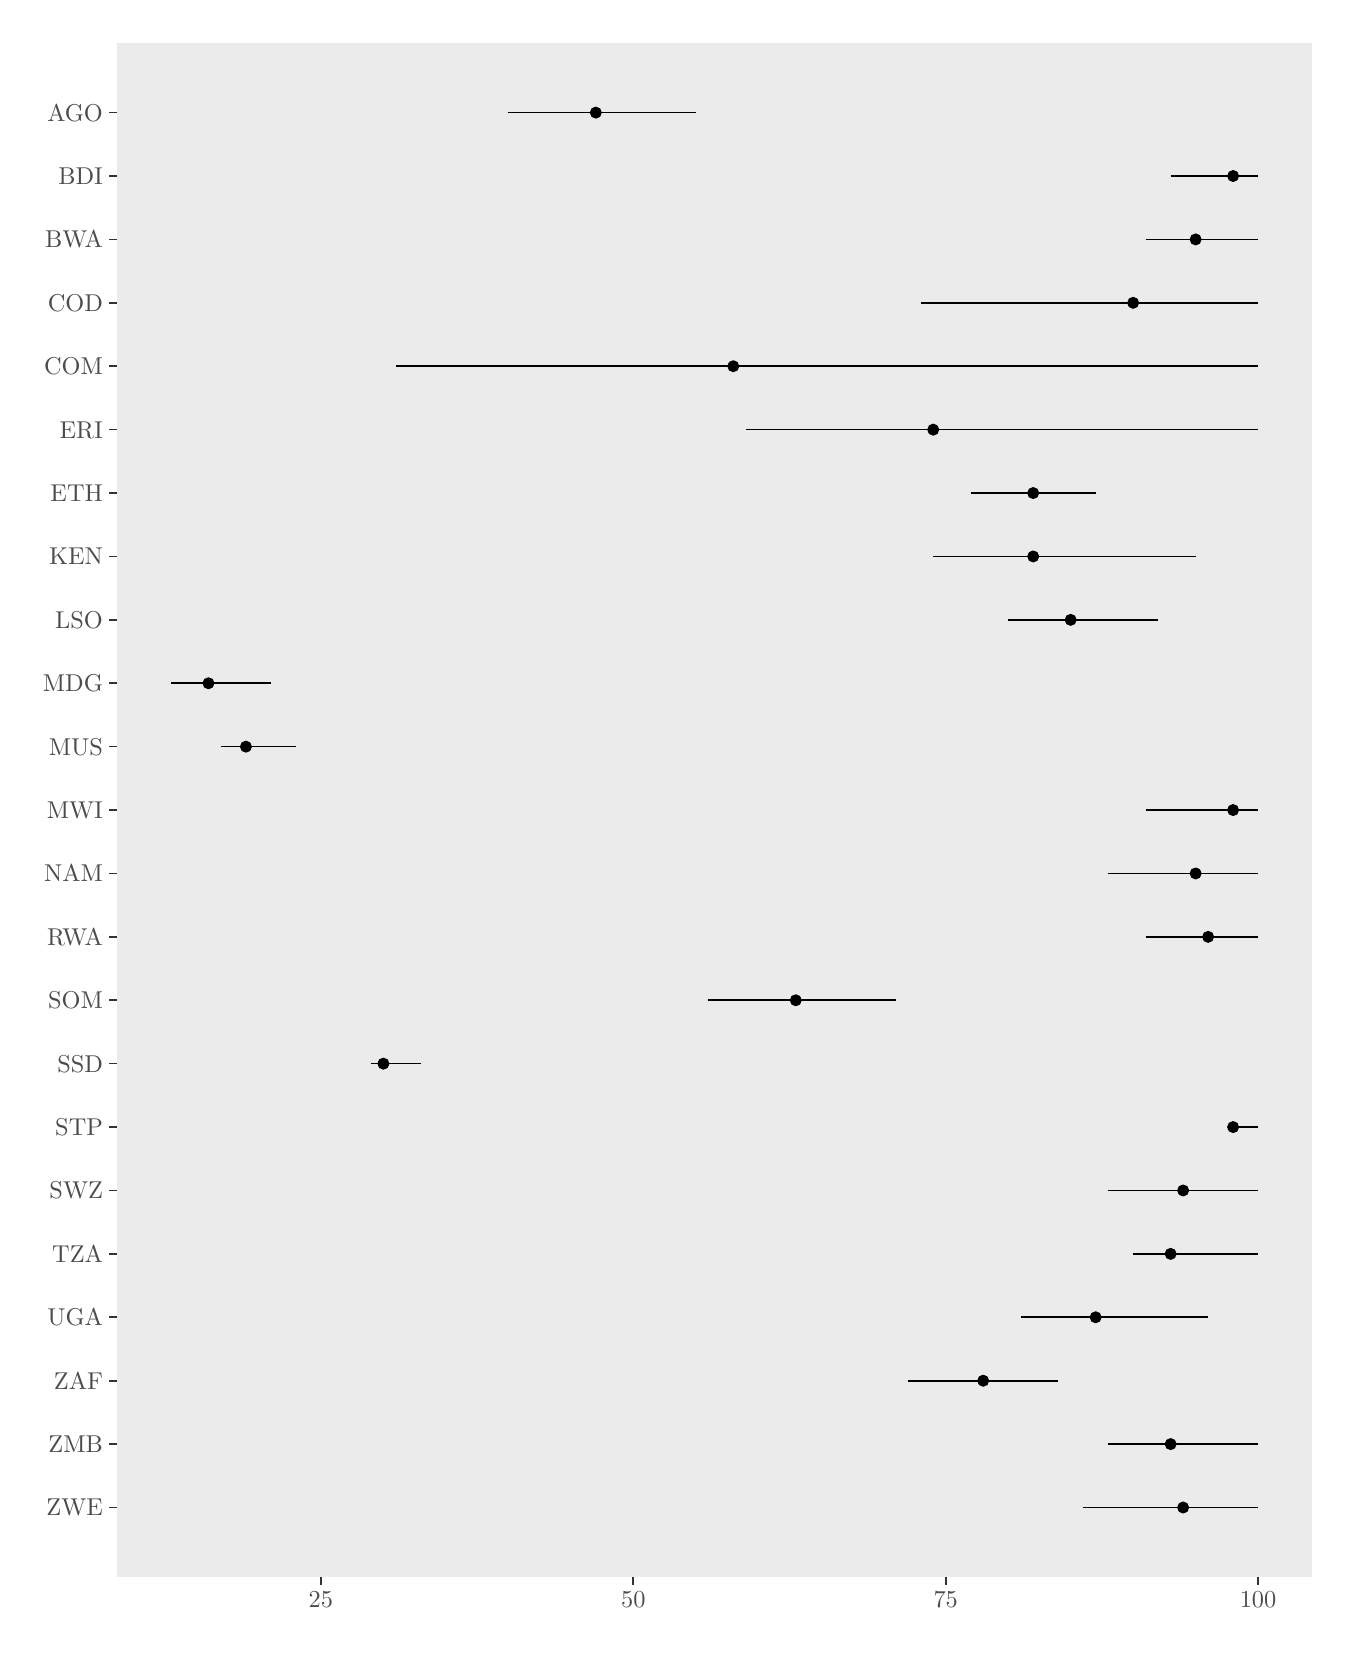
\begin{tikzpicture}[x=1pt,y=1pt]
\definecolor{fillColor}{RGB}{255,255,255}
\path[use as bounding box,fill=fillColor,fill opacity=0.00] (0,0) rectangle (469.75,578.16);
\begin{scope}
\path[clip] (  0.00,  0.00) rectangle (469.75,578.16);
\definecolor{drawColor}{RGB}{255,255,255}
\definecolor{fillColor}{RGB}{255,255,255}

\path[draw=drawColor,line width= 0.6pt,line join=round,line cap=round,fill=fillColor] (  0.00,  0.00) rectangle (469.76,578.16);
\end{scope}
\begin{scope}
\path[clip] ( 32.14, 18.22) rectangle (464.25,572.66);
\definecolor{fillColor}{gray}{0.92}

\path[fill=fillColor] ( 32.14, 18.22) rectangle (464.25,572.66);
\definecolor{drawColor}{RGB}{0,0,0}

\path[draw=drawColor,line width= 0.6pt,line join=round] (173.69,547.46) -- (241.42,547.46);

\path[draw=drawColor,line width= 0.6pt,line join=round] (413.01,524.55) -- (444.61,524.55);

\path[draw=drawColor,line width= 0.6pt,line join=round] (403.98,501.64) -- (444.61,501.64);

\path[draw=drawColor,line width= 0.6pt,line join=round] (322.70,478.73) -- (444.61,478.73);

\path[draw=drawColor,line width= 0.6pt,line join=round] (133.06,455.82) -- (444.61,455.82);

\path[draw=drawColor,line width= 0.6pt,line join=round] (259.49,432.90) -- (444.61,432.90);

\path[draw=drawColor,line width= 0.6pt,line join=round] (340.76,409.99) -- (385.91,409.99);

\path[draw=drawColor,line width= 0.6pt,line join=round] (327.22,387.08) -- (422.04,387.08);

\path[draw=drawColor,line width= 0.6pt,line join=round] (354.31,364.17) -- (408.49,364.17);

\path[draw=drawColor,line width= 0.6pt,line join=round] ( 51.78,341.26) -- ( 87.90,341.26);

\path[draw=drawColor,line width= 0.6pt,line join=round] ( 69.84,318.35) -- ( 96.93,318.35);

\path[draw=drawColor,line width= 0.6pt,line join=round] (403.98,295.44) -- (444.61,295.44);

\path[draw=drawColor,line width= 0.6pt,line join=round] (390.43,272.53) -- (444.61,272.53);

\path[draw=drawColor,line width= 0.6pt,line join=round] (403.98,249.62) -- (444.61,249.62);

\path[draw=drawColor,line width= 0.6pt,line join=round] (245.94,226.71) -- (313.67,226.71);

\path[draw=drawColor,line width= 0.6pt,line join=round] (124.03,203.80) -- (142.09,203.80);

\path[draw=drawColor,line width= 0.6pt,line join=round] (435.58,180.89) -- (444.61,180.89);

\path[draw=drawColor,line width= 0.6pt,line join=round] (390.43,157.98) -- (444.61,157.98);

\path[draw=drawColor,line width= 0.6pt,line join=round] (399.46,135.07) -- (444.61,135.07);

\path[draw=drawColor,line width= 0.6pt,line join=round] (358.82,112.16) -- (426.55,112.16);

\path[draw=drawColor,line width= 0.6pt,line join=round] (318.18, 89.24) -- (372.37, 89.24);

\path[draw=drawColor,line width= 0.6pt,line join=round] (390.43, 66.33) -- (444.61, 66.33);

\path[draw=drawColor,line width= 0.6pt,line join=round] (381.40, 43.42) -- (444.61, 43.42);
\definecolor{fillColor}{RGB}{0,0,0}

\path[draw=drawColor,line width= 0.4pt,line join=round,line cap=round,fill=fillColor] (205.30,547.46) circle (  1.96);

\path[draw=drawColor,line width= 0.4pt,line join=round,line cap=round,fill=fillColor] (435.58,524.55) circle (  1.96);

\path[draw=drawColor,line width= 0.4pt,line join=round,line cap=round,fill=fillColor] (422.04,501.64) circle (  1.96);

\path[draw=drawColor,line width= 0.4pt,line join=round,line cap=round,fill=fillColor] (399.46,478.73) circle (  1.96);

\path[draw=drawColor,line width= 0.4pt,line join=round,line cap=round,fill=fillColor] (254.97,455.82) circle (  1.96);

\path[draw=drawColor,line width= 0.4pt,line join=round,line cap=round,fill=fillColor] (327.22,432.90) circle (  1.96);

\path[draw=drawColor,line width= 0.4pt,line join=round,line cap=round,fill=fillColor] (363.34,409.99) circle (  1.96);

\path[draw=drawColor,line width= 0.4pt,line join=round,line cap=round,fill=fillColor] (363.34,387.08) circle (  1.96);

\path[draw=drawColor,line width= 0.4pt,line join=round,line cap=round,fill=fillColor] (376.88,364.17) circle (  1.96);

\path[draw=drawColor,line width= 0.4pt,line join=round,line cap=round,fill=fillColor] ( 65.33,341.26) circle (  1.96);

\path[draw=drawColor,line width= 0.4pt,line join=round,line cap=round,fill=fillColor] ( 78.87,318.35) circle (  1.96);

\path[draw=drawColor,line width= 0.4pt,line join=round,line cap=round,fill=fillColor] (435.58,295.44) circle (  1.96);

\path[draw=drawColor,line width= 0.4pt,line join=round,line cap=round,fill=fillColor] (422.04,272.53) circle (  1.96);

\path[draw=drawColor,line width= 0.4pt,line join=round,line cap=round,fill=fillColor] (426.55,249.62) circle (  1.96);

\path[draw=drawColor,line width= 0.4pt,line join=round,line cap=round,fill=fillColor] (277.55,226.71) circle (  1.96);

\path[draw=drawColor,line width= 0.4pt,line join=round,line cap=round,fill=fillColor] (128.54,203.80) circle (  1.96);

\path[draw=drawColor,line width= 0.4pt,line join=round,line cap=round,fill=fillColor] (435.58,180.89) circle (  1.96);

\path[draw=drawColor,line width= 0.4pt,line join=round,line cap=round,fill=fillColor] (417.52,157.98) circle (  1.96);

\path[draw=drawColor,line width= 0.4pt,line join=round,line cap=round,fill=fillColor] (413.01,135.07) circle (  1.96);

\path[draw=drawColor,line width= 0.4pt,line join=round,line cap=round,fill=fillColor] (385.91,112.16) circle (  1.96);

\path[draw=drawColor,line width= 0.4pt,line join=round,line cap=round,fill=fillColor] (345.28, 89.24) circle (  1.96);

\path[draw=drawColor,line width= 0.4pt,line join=round,line cap=round,fill=fillColor] (413.01, 66.33) circle (  1.96);

\path[draw=drawColor,line width= 0.4pt,line join=round,line cap=round,fill=fillColor] (417.52, 43.42) circle (  1.96);
\end{scope}
\begin{scope}
\path[clip] (  0.00,  0.00) rectangle (469.75,578.16);
\definecolor{drawColor}{gray}{0.30}

\node[text=drawColor,anchor=base east,inner sep=0pt, outer sep=0pt, scale=  0.88] at ( 27.19,544.43) {AGO};

\node[text=drawColor,anchor=base east,inner sep=0pt, outer sep=0pt, scale=  0.88] at ( 27.19,521.52) {BDI};

\node[text=drawColor,anchor=base east,inner sep=0pt, outer sep=0pt, scale=  0.88] at ( 27.19,498.61) {BWA};

\node[text=drawColor,anchor=base east,inner sep=0pt, outer sep=0pt, scale=  0.88] at ( 27.19,475.70) {COD};

\node[text=drawColor,anchor=base east,inner sep=0pt, outer sep=0pt, scale=  0.88] at ( 27.19,452.79) {COM};

\node[text=drawColor,anchor=base east,inner sep=0pt, outer sep=0pt, scale=  0.88] at ( 27.19,429.87) {ERI};

\node[text=drawColor,anchor=base east,inner sep=0pt, outer sep=0pt, scale=  0.88] at ( 27.19,406.96) {ETH};

\node[text=drawColor,anchor=base east,inner sep=0pt, outer sep=0pt, scale=  0.88] at ( 27.19,384.05) {KEN};

\node[text=drawColor,anchor=base east,inner sep=0pt, outer sep=0pt, scale=  0.88] at ( 27.19,361.14) {LSO};

\node[text=drawColor,anchor=base east,inner sep=0pt, outer sep=0pt, scale=  0.88] at ( 27.19,338.23) {MDG};

\node[text=drawColor,anchor=base east,inner sep=0pt, outer sep=0pt, scale=  0.88] at ( 27.19,315.32) {MUS};

\node[text=drawColor,anchor=base east,inner sep=0pt, outer sep=0pt, scale=  0.88] at ( 27.19,292.41) {MWI};

\node[text=drawColor,anchor=base east,inner sep=0pt, outer sep=0pt, scale=  0.88] at ( 27.19,269.50) {NAM};

\node[text=drawColor,anchor=base east,inner sep=0pt, outer sep=0pt, scale=  0.88] at ( 27.19,246.59) {RWA};

\node[text=drawColor,anchor=base east,inner sep=0pt, outer sep=0pt, scale=  0.88] at ( 27.19,223.68) {SOM};

\node[text=drawColor,anchor=base east,inner sep=0pt, outer sep=0pt, scale=  0.88] at ( 27.19,200.77) {SSD};

\node[text=drawColor,anchor=base east,inner sep=0pt, outer sep=0pt, scale=  0.88] at ( 27.19,177.86) {STP};

\node[text=drawColor,anchor=base east,inner sep=0pt, outer sep=0pt, scale=  0.88] at ( 27.19,154.95) {SWZ};

\node[text=drawColor,anchor=base east,inner sep=0pt, outer sep=0pt, scale=  0.88] at ( 27.19,132.04) {TZA};

\node[text=drawColor,anchor=base east,inner sep=0pt, outer sep=0pt, scale=  0.88] at ( 27.19,109.12) {UGA};

\node[text=drawColor,anchor=base east,inner sep=0pt, outer sep=0pt, scale=  0.88] at ( 27.19, 86.21) {ZAF};

\node[text=drawColor,anchor=base east,inner sep=0pt, outer sep=0pt, scale=  0.88] at ( 27.19, 63.30) {ZMB};

\node[text=drawColor,anchor=base east,inner sep=0pt, outer sep=0pt, scale=  0.88] at ( 27.19, 40.39) {ZWE};
\end{scope}
\begin{scope}
\path[clip] (  0.00,  0.00) rectangle (469.75,578.16);
\definecolor{drawColor}{gray}{0.20}

\path[draw=drawColor,line width= 0.6pt,line join=round] ( 29.39,547.46) --
	( 32.14,547.46);

\path[draw=drawColor,line width= 0.6pt,line join=round] ( 29.39,524.55) --
	( 32.14,524.55);

\path[draw=drawColor,line width= 0.6pt,line join=round] ( 29.39,501.64) --
	( 32.14,501.64);

\path[draw=drawColor,line width= 0.6pt,line join=round] ( 29.39,478.73) --
	( 32.14,478.73);

\path[draw=drawColor,line width= 0.6pt,line join=round] ( 29.39,455.82) --
	( 32.14,455.82);

\path[draw=drawColor,line width= 0.6pt,line join=round] ( 29.39,432.90) --
	( 32.14,432.90);

\path[draw=drawColor,line width= 0.6pt,line join=round] ( 29.39,409.99) --
	( 32.14,409.99);

\path[draw=drawColor,line width= 0.6pt,line join=round] ( 29.39,387.08) --
	( 32.14,387.08);

\path[draw=drawColor,line width= 0.6pt,line join=round] ( 29.39,364.17) --
	( 32.14,364.17);

\path[draw=drawColor,line width= 0.6pt,line join=round] ( 29.39,341.26) --
	( 32.14,341.26);

\path[draw=drawColor,line width= 0.6pt,line join=round] ( 29.39,318.35) --
	( 32.14,318.35);

\path[draw=drawColor,line width= 0.6pt,line join=round] ( 29.39,295.44) --
	( 32.14,295.44);

\path[draw=drawColor,line width= 0.6pt,line join=round] ( 29.39,272.53) --
	( 32.14,272.53);

\path[draw=drawColor,line width= 0.6pt,line join=round] ( 29.39,249.62) --
	( 32.14,249.62);

\path[draw=drawColor,line width= 0.6pt,line join=round] ( 29.39,226.71) --
	( 32.14,226.71);

\path[draw=drawColor,line width= 0.6pt,line join=round] ( 29.39,203.80) --
	( 32.14,203.80);

\path[draw=drawColor,line width= 0.6pt,line join=round] ( 29.39,180.89) --
	( 32.14,180.89);

\path[draw=drawColor,line width= 0.6pt,line join=round] ( 29.39,157.98) --
	( 32.14,157.98);

\path[draw=drawColor,line width= 0.6pt,line join=round] ( 29.39,135.07) --
	( 32.14,135.07);

\path[draw=drawColor,line width= 0.6pt,line join=round] ( 29.39,112.16) --
	( 32.14,112.16);

\path[draw=drawColor,line width= 0.6pt,line join=round] ( 29.39, 89.24) --
	( 32.14, 89.24);

\path[draw=drawColor,line width= 0.6pt,line join=round] ( 29.39, 66.33) --
	( 32.14, 66.33);

\path[draw=drawColor,line width= 0.6pt,line join=round] ( 29.39, 43.42) --
	( 32.14, 43.42);
\end{scope}
\begin{scope}
\path[clip] (  0.00,  0.00) rectangle (469.75,578.16);
\definecolor{drawColor}{gray}{0.20}

\path[draw=drawColor,line width= 0.6pt,line join=round] (105.96, 15.47) --
	(105.96, 18.22);

\path[draw=drawColor,line width= 0.6pt,line join=round] (218.85, 15.47) --
	(218.85, 18.22);

\path[draw=drawColor,line width= 0.6pt,line join=round] (331.73, 15.47) --
	(331.73, 18.22);

\path[draw=drawColor,line width= 0.6pt,line join=round] (444.61, 15.47) --
	(444.61, 18.22);
\end{scope}
\begin{scope}
\path[clip] (  0.00,  0.00) rectangle (469.75,578.16);
\definecolor{drawColor}{gray}{0.30}

\node[text=drawColor,anchor=base,inner sep=0pt, outer sep=0pt, scale=  0.88] at (105.96,  7.21) {25};

\node[text=drawColor,anchor=base,inner sep=0pt, outer sep=0pt, scale=  0.88] at (218.85,  7.21) {50};

\node[text=drawColor,anchor=base,inner sep=0pt, outer sep=0pt, scale=  0.88] at (331.73,  7.21) {75};

\node[text=drawColor,anchor=base,inner sep=0pt, outer sep=0pt, scale=  0.88] at (444.61,  7.21) {100};
\end{scope}
\end{tikzpicture}

\caption{Point estimates and plausible intervals shown in Table~\ref{tab_data}.}
\label{fig_data}
\end{figure}

We now turn away from simulations and into the analysis of real data.  We will examine a data set drawn from the World Bank Gender Statistics Database~\citep{worldBankData} describing what percentage of the female population of countries in Southern and Eastern Africa had access to anti-retroviral drugs in 2021 (series code SH.HIV.ARTC.FE.ZS).  For each country, the data set includes a point estimate and a range of plausible values.  The data are reported in percentage points rounded to the nearest integer.

We begin with a presentation of the data.  Table~\ref{tab_data} shows the point estimates and plausible intervals for each country.  Two countries (Mozambique and Seychelles) are excluded for missing data.  Table~\ref{tab_data} also shows the sample ranks, rank intervals and sample interval order ranks.  Although the sample ranks are numerically quite different from the sample interval order ranks, the normalized distance between the orders they define is only approximately \dataRankDistance.

The symmetrized and normalized average excess for this set of interval estimates is \dataUncertainty.  Because the interval estimate for Comoros is exceptionally wide and intersects a large number of other intervals, we might expect that it is driving the uncertainty to a large degree.  If we exclude it, the symmetrized and normalized average excess drops to \dataSubsetUncertainty.  Omitting any other country's record leads either to a smaller decrease or an increase.  The difference between the total rank uncertainty and the rank uncertainty omitting a given set of records may be a useful measure of how influential that subset is in some sense.

The point estimates and plausible intervals from Table~\ref{tab_data} are also shown in Figure~\ref{fig_data}.  The figure makes it clear that Madagascar and Mauritius are estimated to rank below all the other countries regardless of the actual values of the rank estimates.  We see a similar pattern in the data considered in~\cite{klein2020jointCR} where there are values that separate groups of intervals, and this topic deserves further consideration.

I do not recommend plotting the rank intervals as was done in~\cite{klein2020jointCR} because it is difficult to determine the order relation by visually examining them.  Even for the small order shown in Table~\ref{tab_rank_int_counter} it would take some care to determine that $1 < 4$ given only the rank intervals.

\bibliographystyle{apalike}
\bibliography{OrderPerspRankEst}

\end{document}
